% =====================================================================
% Ranking Is Not Deliverable Capacity:
% Operational Calibration and Stress Testing in a Sichuan-Informed
% Demand-Response Benchmark
%
% Target: Frontiers in Energy Research
% =====================================================================

\documentclass[utf8]{FrontiersinHarvard}

\usepackage{url,hyperref,lineno,microtype,subcaption}
\usepackage[onehalfspacing]{setspace}
\usepackage{algorithm}
\usepackage{algpseudocode}
\usepackage{booktabs}
\usepackage{multirow}
\usepackage{amsmath,amssymb}
\usepackage{graphicx}

\linenumbers

% --- Custom commands ---
\newcommand{\trueval}{\tau_{\mathrm{true}}}
\newcommand{\tauhat}{\hat{\tau}}
\newcommand{\pehe}{\mathrm{PEHE}}
\newcommand{\Mhat}{\widehat{M}}
\newcommand{\Moracle}{M^{\mathrm{oracle}}}
\newcommand{\Preq}{P^{\mathrm{req}}}
\newcommand{\Pcommit}{P^{\mathrm{commit}}}
\newcommand{\Pdeliv}{P^{\mathrm{deliv}}}
\newcommand{\Shortfall}{\mathrm{Shortfall}}
\newcommand{\OCR}{\mathrm{OCR}}
\newcommand{\TSR}{\mathrm{TSR}}
\newcommand{\UAR}{\mathrm{UAR}}

\def\keyFont{\fontsize{8}{11}\helveticabold }
\def\firstAuthorLast{Zhang {et~al.}}
\def\Authors{Ling Zhang\,$^{1}$, Bowei Yang\,$^{1}$, Xingsi Ke\,$^{1}$, Hong Zhao\,$^{1}$, Wenhua Zhang\,$^{1}$ and Yumin Yao\,$^{2,*}$}
\def\Address{$^{1}$State Grid Sichuan Electric Power Corporation, Chengdu, Sichuan, China \\
$^{2}$Central South University, Changsha, China}
\def\corrAuthor{Yumin Yao}
\def\corrEmail{yaoyumin@csu.edu.cn}

\begin{document}
\onecolumn
\firstpage{1}

\title[Ranking Is Not Deliverable Capacity]{Ranking Is Not Deliverable Capacity: Operational Calibration and Stress Testing in a Sichuan-Informed Demand-Response Benchmark}

\author[\firstAuthorLast ]{\Authors}
\address{\Address}
\correspondance{\corrAuthor\\\corrEmail}

\extraAuth{}

\maketitle

\begin{abstract}
\section{}
Sichuan's fine-grained load-management programme has assembled a
regulatable resource library of approximately 9\,GW. As of July
2025, 26 virtual power plants (VPPs) had been connected to the
provincial dispatch platform. Yet the registered nameplate
capacity of a resource is not the capacity it can reliably
deliver under a specific demand-response task. We formalise this
gap as a task-conditioned deliverable capacity estimation
problem: given a task with required reduction~$\Preq$, a
platform must select a subset of resources and commit
an aggregate capacity that will actually be delivered.
Using a Sichuan-informed benchmark generated through paired
routine- and stress-regime interventions
(1{,}950 users, five demand-response tasks, 9{,}750 user--task
assessments, three anonymized city settings, and an execution
realization factor mean-anchored to PJM's reported 67\%
delivery ratio and plausibility-checked against MISO, NYISO,
and other empirical studies), we show that a capacity-based heuristic
retains strong ranking ability
(Spearman $\rho \approx 0.89$) but produces only
\textbf{42.9\% task success rate} (seed-clustered
bootstrap 95\% CI: 39.8--46.0\%) at the $5\times$ scaled requirement across
$N=30$ independent benchmark realizations.
In contrast, a simple global linear calibration achieves
$87.3\%$ (95\% CI: 84.4--90.0\%) task success, indicating
that ranking becomes operationally useful only when the predicted
quantity is expressed on an appropriate deliverable-capacity scale.
A split-conformal lower-bound estimator further raises task
success to $95.3\%$ (empirical coverage 90.1\%; $N=30$ seeds)
while selecting only
$1.5\times$ more
resources than the uncalibrated heuristic.
Under a standardized severe stress contrast,
even the routine-regime oracle achieves only
$3.6\%$ task success at $5\times$, demonstrating a substantial
routine-to-stress transfer gap; only deliberately conservative
estimation maintains $75.1\%$ TSR under cross-regime stress.
We propose operational replay metrics---task success rate (TSR),
over-commit rate (OCR), and full-pool feasibility---that directly
measure the business consequences of estimation error, and argue
that fine-grained load management requires calibrated
kW-level capacity estimates, not just effect rankings.

\tiny
 \keyFont{ \section{Keywords:} demand response; fine-grained load management; deliverable capacity estimation; ranking--calibration gap; execution realization factor; stress-test extrapolation; task-level operational replay; virtual power plant; Sichuan power grid}
\end{abstract}

% BODY TEXT WILL BE INSERTED HERE
% NOTE: \cite changed to \citep for Frontiers Harvard style
%       figure* changed to figure with [h!] placement
%       \includegraphics changed to direct callouts per Frontiers template
%       Tables moved to end per Frontiers requirement

\section{Introduction}
\label{sec:intro}

Sichuan's electricity demand-response system has evolved from
broad-brush ordered consumption curtailment toward task-level,
parameterised load management. The national \emph{Measures for
the Management of Electrical Load}~\citep{ndrc2023loadmgmt}
codifies the full business chain---eligibility verification,
capability assessment, response invitation, process monitoring,
and effect evaluation---and requires implementation through
the new-type power-load management system. The provincial
load-management centre, established in 2023 at the city,
prefecture, and county levels, registers each participating
user's maximum and minimum responsive capacity, minimum
response duration, and available time windows. By July 2025,
Sichuan reported a regulatable resource library of
approximately 9\,GW and 26 virtual power plants (VPPs)
connected to the provincial operational platform with a
combined adjustable capability of roughly 900\,MW.
The national VPP development
guidance~\citep{ndrc2025vppguide} further accelerates this
trajectory. The 2026 provincial demand-side market response
implementation requires 96-point daily load-curve telemetry
and formal declaration of response parameters from all
participants.
A recent industry report on Chinese industrial demand-side
flexibility~\citep{rmi2023china} similarly highlights that the
technical potential for DR is large but that converting it into
reliable commitment is the binding operational challenge.

This expansion creates a critical operational tension. The
resource library is large, but the capacity that any given
resource can \emph{reliably deliver under a specific task} is
smaller than its registered nameplate rating---sometimes
dramatically so. Empirical evidence from multiple independent
system operators confirms this gap: PJM demand-response
resources delivered an average of only 67\% of committed
capacity during summer 2025 events, with performance dropping
to 26--32\% during Winter Storm
Elliott~\citep{pjm2026marketmonitor,recurve2026elliott}.
NYISO Special Case Resources show response rates of
51--92\% depending on load zone and hour~\citep{nyiso2026scr},
and Korean residential programs exhibit 83\% customer-level
overestimation under common baseline
methods~\citep{kim2018freerider}. These findings motivate the
execution realization factor~$\xi$ adopted in our benchmark
(Section~\ref{subsec:dose_response}).
A platform that commits based on registered
capacity risks over-promising; one that selects resources based
on ranking alone does not know how many kilowatts it can safely
pledge. The central business question is not ``can this user
respond?'' but ``\textbf{under task condition~$q_t$, how many
kilowatts can this resource reliably deliver, and how much
backup must the platform hold?}''

This question sits between capability verification and portfolio
commitment in the load-management workflow. It is not a complete
VPP dispatch optimiser, a market clearing engine, or a real-time
controller. Rather, it is the decision-support module that
converts a pool of candidate resources into a reliable capacity
commitment.

\textbf{Our central claim can be stated in one sentence:}
\begin{quote}
\textit{Ranking determines whom to call; calibration determines
how much capacity can be safely committed.}
\end{quote}

To support this investigation, we use a platform-informed
paired-intervention benchmark that represents user resources,
task requirements, operational context, and violation-induced
delivery degradation. For each user--task instance, the benchmark
contains a routine-regime outcome and a counterfactual outcome
under a fixed standardized severe stress contrast. The two
outcomes share the same user--task context and exogenous execution
noise and differ only in the intervention state. This design
provides oracle quantities for examining both relative resource
ordering and absolute deliverable-capacity calibration.

Building on this paired-intervention design, the present study
formalises and quantifies the gap between resource-ranking
ability and capacity-commitment reliability. We define
task-level operational replay metrics that measure the business
consequences of estimation error and examine how individual-level
magnitude bias propagates into portfolio shortfalls,
over-commitment, and task failure.

\textit{Position in the literature.} Existing demand-response
studies have separately investigated heterogeneous response
estimation~\citep{zhou2017estimating,li2017linear,he2024behavior},
participant targeting~\citep{antonopoulos2021data}, flexibility
forecasting~\citep{hekmat2021flexibility,hybrid2025flexforecast},
and uncertainty-aware VPP
bidding~\citep{naughton2021cooptimizing,zhang2023distributionally,vpp2025credible}.
Calibration methods for aggregate flexibility have also
appeared~\citep{conformal2026prosumer,prakobkaew2025selection}.
However, limited attention has been paid to the operational
interface between individual-level ranking and aggregate
capacity commitment. A model may rank resources accurately
while systematically overstating their deliverable kW capacity,
causing the selection process to accumulate optimistic errors
and produce portfolio-level shortfalls. This study addresses
that gap through task-level operational replay under routine
and stress regimes (Sections~\ref{sec:related}--\ref{sec:scenario}).
Figure~\ref{fig:ranking_not_capacity} illustrates the central
ranking--calibration distinction examined in this study.
A model may preserve the relative priority of candidate resources
while systematically overstating their deliverable capacity in kW.
Consequently, the ranking remains informative for determining whom
to call, but the magnitude bias accumulates during portfolio
construction and can cause the committed capacity to exceed the
realized aggregate delivery.

This distinction motivates an operational evaluation that extends
beyond individual-level rank correlation.
We replay the complete commitment process and examine whether the
selected portfolio can satisfy the requested capacity under both
routine and severe stress regimes.

\begin{figure}[h!]
\begin{center}
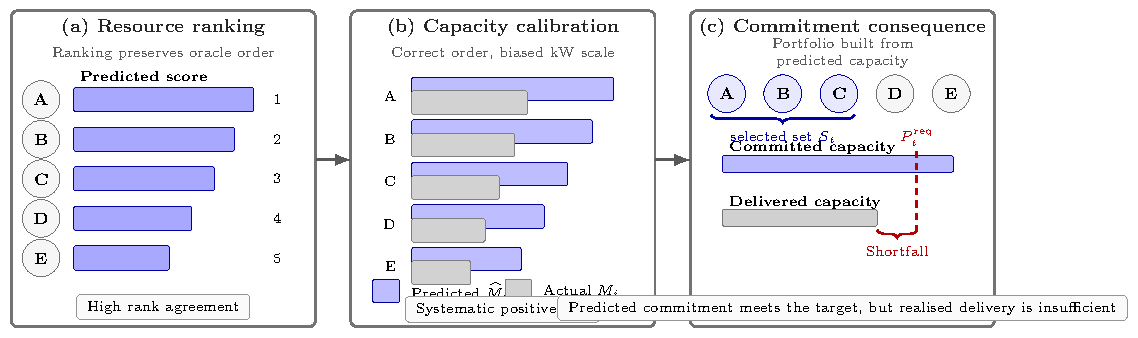
\includegraphics[width=12cm]{figures/fig1_ranking_not_capacity}
\end{center}
\caption{Conceptual distinction between resource ranking and
deliverable-capacity calibration. A model may preserve the relative
ordering of candidate resources while systematically overestimating
their deliverable capacity. When the biased predictions are used for
portfolio construction, the predicted commitment can satisfy the
task requirement even though the realized delivery remains
insufficient.}\label{fig:ranking_not_capacity}
\end{figure}



\textbf{Contributions.} This paper makes four contributions:
\begin{enumerate}
    \item \textit{Business formulation.} We formalise Sichuan's
    fine-grained load-management capacity-verification and
    task-commitment problem as a task-conditioned deliverable
    capacity estimation problem, bridging the gap between
    resource-pool ranking and reliable capacity commitment
    (Sections~\ref{sec:workflow}--\ref{sec:formulation}).

    \item \textit{Dual-regime diagnosis.} We separate the
    observational-regime oracle ($\tau^{\mathrm{regime}}$) from
    the stress-test oracle ($\tau^{\mathrm{stress}}$) and show
    that the ranking--calibration gap decomposes into a
    dose-extrapolation component (ratio of mean absolute effects
    $\approx 32\times$; median paired instance-level ratio
    $\approx 91.7\times$) and a ranking-mismatch component (Spearman~0.327
    between regimes)
    (Section~\ref{sec:effect_results}).

    \item \textit{Shortcut and calibration analysis.} We show
    that resource capacity and a small number of operational
    features achieve high Spearman ranking correlation
    ($\rho \approx 0.89$ on the full benchmark) but
    cannot guarantee task-level capacity accuracy, and that
    calibration raises task success rates
    from 42.9\% to 87.3\% at the $5\times$ scaled requirement,
    with a split-conformal lower-bound estimator further
    raising it to 95.3\%
    (Section~\ref{sec:replay}).

    \item \textit{Operational replay.} We propose
    task-level replay metrics (TSR, OCR, full-pool feasibility)
    and demonstrate, across 3~cities, 5~tasks, 4~requirement
    levels, and $N=30$ independent benchmark realizations, that
    a capacity-based heuristic with strong ranking
    ($\rho \approx 0.89$) produces only 42.9\% task success at the
    $5\times$ scaled requirement, while global linear calibration with
    similar ranking achieves 87.3\%---showing
    that ranking becomes operationally useful only when paired
    with appropriate kW-scale calibration. Under cross-regime
    stress, even the routine-regime oracle achieves only 3.6\%
    TSR at $5\times$, demonstrating
    a substantial dose-extrapolation limitation
    (Sections~\ref{sec:replay}--\ref{sec:scenario}).
\end{enumerate}


\section{Related Work}
\label{sec:related}

Existing research related to this paper spans four largely
independent strands. We review each, identify the interface
this paper addresses, and articulate the gap.

\subsection{Heterogeneous Response Estimation and Targeting}
\label{subsec:rw_hte}

A first strand estimates heterogeneous demand-response effects
from experimental or observational data and uses them to target
high-response users. \citep{zhou2017estimating} use causal
decision trees on approximately 7{,}000 California residential
customers to identify heterogeneous hour-level price effects and
improve targeting cost-efficiency.
\citep{li2017linear} compare linear regression, covariate
interaction, and modified-covariate methods for DR treatment
effect estimation, showing that adding user features does not
necessarily improve estimation---the key lies in modelling
treatment--covariate interactions.
\citep{he2024behavior} introduce X-learner, R-learner, and
doubly-robust learners into DR behavior assessment, enabling
ex-ante policy evaluation.
\citep{antonopoulos2021data} model response behavior from a
large-scale residential trial using machine learning, revealing
strong temporal and behavioral heterogeneity.
Recent work has also extended the targeting literature to
individual-level potential evaluation
\citep{jiao2023individual} and to systematic reviews of
forecasting methods~\citep{muqtadir2025drpotential}, while
end-to-end deep learning frameworks can jointly identify
response models and estimate customer baselines
\citep{chen2021endtoend}.

These studies answer ``\textit{who responds more?''} but rarely
ask ``\textit{if we select these users, can the portfolio
deliver the required aggregate capacity?''} The interface
between individual-level effect estimation and portfolio-level
commitment reliability remains unexamined.

\subsection{Demand-Side Flexibility Quantification}
\label{subsec:rw_flex}

A second strand forecasts user or aggregate flexibility.
\citep{hekmat2021flexibility} propose data-driven prediction
of flexibility envelopes---time-coupled bounds on adjustable
load---arguing that flexibility cannot be represented by a
single static capacity value.
The hybrid forecasting framework of
\citep{hybrid2025flexforecast} combines probabilistic load
prediction with virtual battery models to estimate event-period
reduction and post-event rebound. These works highlight that
nameplate load and deliverable response capacity differ
substantially across user types and operating conditions.
A growing body of work focuses specifically on day-ahead DR
potential forecasting under dynamic spatial-temporal
correlations~\citep{li2023dayahead} and on industrial users,
where flexibility is governed by production processes rather
than discretionary load shifting
\citep{lu2021industrial,santecchia2022flexibility,sieving2026idrrc}.

This literature establishes that deliverable capacity is a
task-conditioned function $M_i(q_t, X_i)$, not a fixed
attribute---a premise this paper adopts. However, these studies
focus on forecasting accuracy at the individual or aggregate
level; they do not analyse how individual-level prediction
errors propagate through greedy resource selection into
portfolio-level shortfalls.

\subsection{Uncertainty-Aware VPP Bidding and Credible Capacity}
\label{subsec:rw_vpp}

A third strand optimises VPP bidding and dispatch under
resource and market uncertainty.
\citep{naughton2021cooptimizing} co-optimise VPP energy and
ancillary service offerings under renewable uncertainty.
\citep{wang2023vppreview} survey VPP uncertainty management,
noting that stochastic, robust, and distributionally robust
optimization methods all address the fundamental gap between
committed and actual delivery.
\citep{zhang2023distributionally} formulate a two-stage
distributionally robust VPP bidding model for joint energy and
flexible ramping products, controlling declaration conservatism
via Wasserstein ambiguity sets.
\citep{vpp2025credible} evaluate VPP credible capacity using
probabilistic forecasting and CVaR-based reliability metrics,
emphasising that predicted capacity must be converted to a
conservative, reliability-calibrated commitment.
Recent work has extended this literature to coordinated
aggregation and disaggregation with the distribution network
operator~\citep{liu2024vppaggregation} and to load-aggregation
scheduling for specific VPP configurations such as port
adjustable resources~\citep{zhang2025vppscheduling}. A recent
survey of C\&I DR flexibility with energy storage and renewable
sources further contextualises the role of VPPs in the broader
flexibility stack~\citep{yasmin2024survey}.

These studies share our premise that
$\Pcommit \neq \Pdeliv$. However, they typically treat the
resource capability model as given---focusing on how to
\emph{optimise bidding given a capability model}---rather than
auditing whether the capability model itself is sufficiently
calibrated to support a reliable commitment. This paper
provides that audit: we show that a model with high ranking
accuracy ($\rho \approx 0.89$) can produce systematically unreliable
commitments.

\subsection{Reliable Aggregation and Calibration}
\label{subsec:rw_calib}

A fourth strand develops calibration methods for aggregate
resource commitments.
\citep{conformal2026prosumer} combine Monte Carlo dropout
with conformal prediction to produce finite-sample calibrated
intervals for prosumer flexibility aggregation, showing that
uncalibrated models systematically overbid and violate
market reliability requirements (e.g., P90 coverage).
\citep{prakobkaew2025selection} compare participant-selection
strategies for DR load aggregation---duration-based,
price-based, and forecast-based---in a Thai pilot, finding that
dual-forecast selection reduces operational cost and the number
of users called.
Conformal and probabilistic calibration methods have
increasingly been applied to energy and electricity price
forecasting~\citep{oconnor2025conformal}, while customer
baseline load (CBL) estimation has been a long-standing
prerequisite for incentive-based DR settlement
\citep{park2015cbl,li2025cbl}.

The conformal calibration work is closest in spirit to our
ConservativeQ10 strategy: both convert raw predictions into
reliability-aware lower bounds. However, that work calibrates
the \emph{aggregate} forecast directly; our work analyses how
the \emph{selection mechanism} itself---ranking users by
predicted capacity---accumulates optimistic errors at the
portfolio level, and how this accumulation differs between
routine and stress regimes.

\textit{Summary.} The four strands address targeting
(Section~\ref{subsec:rw_hte}), flexibility forecasting
(\ref{subsec:rw_flex}), bidding optimization
(\ref{subsec:rw_vpp}), and calibration
(\ref{subsec:rw_calib}). Limited prior work has explicitly evaluated the complete chain from individual-level capacity prediction through resource selection and commitment to realized portfolio delivery. This paper occupies that position.


\section{Sichuan Fine-Grained Load-Management Workflow}
\label{sec:workflow}

The Sichuan demand-response business chain comprises eight stages,
from initial resource registration through settlement. We describe
each stage and identify where the task-conditioned capacity
estimation module---the subject of this paper---fits into the
overall workflow.

\subsection{Resource Registration and Parameter Declaration}

Participating users register with the provincial load-management
platform, declaring their industry type, nominal capacity
($P_i^{\mathrm{nom}}$), response ramp rate, availability windows,
and historical demand-response participation. The platform
constructs a resource library indexed by
$(\mathrm{city}, \mathrm{user\_id})$ and maintains a dynamic
record of each resource's operational state.

\subsection{Capability Verification}

Before a resource is admitted to the response pool, the platform
performs capability verification: a technical assessment of
whether the resource's declared capacity is physically achievable
under its operational constraints (production schedule, equipment
limits, comfort thresholds, contractual obligations). Resources
that pass verification are assigned a
\texttt{reliable\_deliverable\_capacity\_kw} rating, which serves
as the platform's baseline estimate of the resource's
deliverable capacity.

This rating is a \emph{steady-state} assessment. It does not
account for task-specific conditions (time of day, event intensity,
duration, simultaneous violations) that may reduce actual delivery
below the rated level.

\subsection{Task Generation and Response Invitation}

The platform issues demand-response tasks parameterised by:
\begin{equation}
    q_t = \bigl[\Preq_t,\; t_s,\; t_e,\; D_t,\;
    r_t^{\mathrm{req}},\; \eta_t^{\mathrm{rel}}\bigr],
    \label{eq:task_def}
\end{equation}
where $\Preq_t$ is the required aggregate capacity reduction
(kW), $t_s$ and $t_e$ are the start and end times, $D_t$ is the
required duration, $r_t^{\mathrm{req}}$ is the minimum response
rate, and $\eta_t^{\mathrm{rel}}$ is the reliability requirement.

\subsection{Task-Conditioned Capacity Estimation}
\label{subsec:capacity_estimation}

\textbf{This is the module this paper addresses.} For each
candidate resource $i$ in the task pool, the platform must
estimate:
\begin{equation}
    \Mhat_i(q_t) = \text{predicted deliverable capacity under
    task~} q_t,
\end{equation}
and use these estimates to select a resource subset
$\mathcal{S}_t$ whose aggregate predicted capacity meets the
requirement:
\begin{equation}
    \sum_{i \in \mathcal{S}_t} \Mhat_i(q_t) \geq \Preq_t.
\end{equation}

The platform then commits
$\Pcommit = \sum_{i \in \mathcal{S}_t} \Mhat_i(q_t)$ to the
dispatch system. At task execution, each resource delivers an
actual amount $M_i(q_t)$, yielding an actual aggregate delivery
$\Pdeliv = \sum_{i \in \mathcal{S}_t} M_i(q_t)$.

The gap between $\Pcommit$ and $\Pdeliv$---and the resulting
capacity shortfall---is the primary quantity this paper
diagnoses and seeks to mitigate.

\subsection{Portfolio Commitment and Dispatch}

Once the resource subset is selected, the platform issues
response invitations, aggregates the committed capacity into a
portfolio bid (for market-based response) or a dispatch order
(for administrative response), and sets backup reserves based
on the reliability target $\eta_t^{\mathrm{rel}}$.

\subsection{Execution Monitoring, Assessment, and Settlement}

During execution, the platform monitors real-time delivery,
flags shortfalls, and records outcomes for post-task assessment
and settlement. Resources that consistently under-deliver may be
reclassified or removed from the pool.

\subsection{Position of This Paper}

Figure~\ref{fig:workflow_positioning} positions the proposed
method within the broader fine-grained load-management
workflow. The upstream process maintains a verified response
resource pool and defines the task requirements, while the
downstream process performs response invitation, execution
monitoring, evaluation, and settlement. This study focuses on
the intermediate commitment-support layer. Given the
registered resource features $X_i$ and task vector $\mathbf{q}_t$,
the module estimates deliverable capacity $\Mhat_i(\mathbf{q}_t)$,
selects a resource portfolio $\mathcal{S}_t$, and produces the
aggregate commitment $P_t^{\mathrm{commit}}$.

Operationally, ranking determines which resources should be called,
whereas deliverable-capacity calibration determines how much
capacity can be safely committed.

\begin{figure}[h!]
\begin{center}
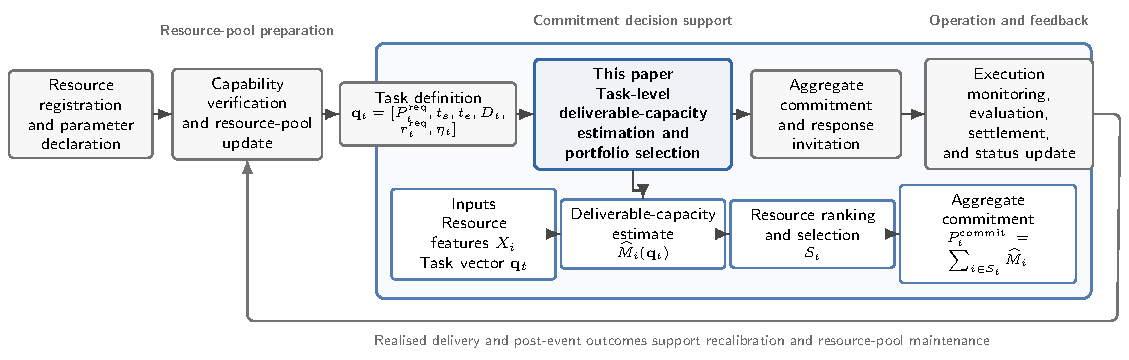
\includegraphics[width=14cm]{figures/fig2_workflow}
\end{center}
\caption{Positioning of the proposed decision-support module in the
fine-grained load-management workflow. The upstream stages maintain
and verify the response resource pool and define task requirements.
The proposed module estimates resource-level deliverable capacity,
ranks and selects candidate resources, and produces an aggregate
commitment. Realised delivery and post-event outcomes are fed back
for model recalibration and resource-pool maintenance.}\label{fig:workflow_positioning}
\end{figure}




\section{Problem Formulation}
\label{sec:formulation}

\subsection{Notation}

Table~\ref{tab:notation} defines the principal symbols used
in this paper.

\begin{table}[h!]
\centering
\caption{Notation summary.}
\label{tab:notation}
\small
\begin{tabular}{llll}
\toprule
\textbf{Symbol} & \textbf{Unit} & \textbf{Definition} & \textbf{Type} \\
\midrule
$P_i^{\mathrm{nom}}$ & kW & Nominal connected capacity & Synthetic input \\
$P_i^{\mathrm{rated}}$ & kW & Benchmark platform-rating proxy & Synthetic input \\
$q_t$ & --- & Task parameter vector & Context \\
$M_i(q_t)$ & kW & Benchmark-realized deliverable capacity & Simulated outcome \\
$\Mhat_i(q_t)$ & kW & Predicted deliverable capacity & Model output \\
$Y_i(\mathbf{0})$ & kW & No-violation delivery & Oracle outcome \\
$\tau_i$ & kW & Violation-induced delivery loss ($\leq 0$) & Oracle estimand \\
$r_i$ & --- & Response rate (dimensionless) & Synthetic input \\
$\xi_{i,t}$ & --- & Execution realization factor ($\in (0,1]$) & Synthetic input \\
$\mathcal{S}_t$ & --- & Selected portfolio & Decision output \\
$\Preq_t$ & kW & Required aggregate capacity reduction & Task parameter \\
$\Pcommit$ & kW & Committed capacity & Replay output \\
$\Pdeliv$ & kW & Realized portfolio delivery & Replay outcome \\
$\Shortfall$ & kW & Capacity deficit & Operational metric \\
$\OCR$ & --- & Over-commit rate & Operational metric \\
$\TSR$ & --- & Task success indicator (binary) & Operational metric \\
$F_{c,t}^{(r)}$ & --- & Full-pool feasibility ratio & Diagnostic \\
\bottomrule
\end{tabular}
\end{table}

Let $\mathcal{U}_c$ denote the set of registered users in city
$c$, and $\mathcal{T}$ the set of task templates. Each
task--city combination $(c, t)$ defines a candidate resource pool
$\mathcal{U}_{c,t} \subseteq \mathcal{U}_c$ of users assessed
under task~$t$.

Each user $i$ has a nominal capacity $P_i^{\mathrm{nom}}$ and a
response rate $r_i$. Under task~$q_t$, the user's actual
deliverable capacity is:
\begin{equation}
    M_i(q_t) = \max\!\bigl(0,\;\; g_\Theta(C_i,\,
    \mathbf{V}_i,\,     U_{i,t})\bigr),
\end{equation}
where $g_\Theta$ is the platform-informed simulator response
function specified in Section~\ref{subsec:dose_response},
$C_i$ is the user--task context, $\mathbf{V}_i$ is the
intervention state, and $U_{i,t}$ denotes shared exogenous execution
noise.

\subsection{Deliverable Capacity and Delivery Loss}

It is convenient to decompose the deliverable capacity into a
baseline (no-violation) component and a violation-induced loss:
\begin{equation}
    M_i(q_t) = Y_i(\mathbf{0}) + \tau_i,
\end{equation}
where $Y_i(\mathbf{0})$ is the delivery under no violation and
$\tau_i \leq 0$ is the violation-induced delivery loss.
The non-positive sign of $\tau_i$ is imposed by benchmark
design ($w_k \leq 0$ for all delivery-affecting classes),
not merely observed empirically; positive violation effects
are excluded by construction.
The
benchmark supports estimation of the violation-induced effect
$\tau_i$; however, the operational quantity required for
capacity commitment is the absolute deliverable capacity $M_i$,
not $\tau_i$ in isolation.

\subsection{Dual-Regime Estimands}

The benchmark provides two distinct oracle estimands:

\textit{Routine-regime oracle:}
\begin{equation}
    \tau_i^{\mathrm{regime}} = Y_i(\mathbf{V}_i^{\mathrm{obs}})
    - Y_i(\mathbf{0}),
\end{equation}
where $\mathbf{V}_i^{\mathrm{obs}}$ is the user's typical
observational violation state.

\textit{Stress-test oracle:}
\begin{equation}
    \tau_i^{\mathrm{stress}} = Y_i(\mathbf{V}^{\mathrm{stress}})
    - Y_i(\mathbf{0}),
\end{equation}
where $\mathbf{V}^{\mathrm{stress}}$ is the fixed standardized severe stress contrast
(all five violation classes active, severity$=$1.0, scope$=$0.5).

The stress-regime delivery is reconstructed via the exact
dual-oracle method:
\begin{equation}
    M_i^{\mathrm{stress}} = Y_i(\mathbf{0}) +
    \tau_i^{\mathrm{stress}},
    \label{eq:stress_reconstruction}
\end{equation}
where $Y_i(\mathbf{0}) = M_i^{\mathrm{routine}} -
\tau_i^{\mathrm{regime}}$.

\subsection{Task-Level Operational Metrics}
\label{subsec:metrics}

Given a requirement $\Preq_t$ and a selection strategy that
produces predicted capacities $\{\Mhat_i\}$, the platform selects
the smallest subset $\mathcal{S}_t$ (ranked by $\Mhat_i$
descending) such that $\sum_{i \in \mathcal{S}_t} \Mhat_i \geq
\Preq_t$.

We define operational metrics:

\begin{equation}
    \Pcommit = \textstyle\sum_{i \in \mathcal{S}_t} \Mhat_i,
    \qquad
    \Pdeliv = \textstyle\sum_{i \in \mathcal{S}_t} M_i,
\end{equation}

\begin{equation}
    \Shortfall = \max(0,\; \Preq - \Pdeliv),
    \qquad
    \OCR = \frac{\max(0,\; \Pcommit - \Pdeliv)}{\Pcommit},
\end{equation}

\begin{equation}
    \TSR = \mathbb{I}(\Pdeliv \geq \Preq).
\end{equation}

These metrics measure the \emph{business consequences} of
estimation error: $\Shortfall$ is the capacity deficit (kW),
$\OCR$ is the fraction of committed capacity that was not
delivered, and $\TSR$ is the binary task success indicator.
We additionally define the full-pool feasibility ratio for
regime $r \in \{\mathrm{routine}, \mathrm{stress}\}$:
\begin{equation}
    F_{c,t}^{(r)} = \frac{\sum_{i \in \mathcal{U}_{c,t}}
    M_i^{(r)}}{\Preq_{c,t}}, \qquad
    \mathrm{Feasible}_{c,t}^{(r)} = \mathbb{I}\!\bigl(F_{c,t}^{(r)} \geq 1\bigr).
\end{equation}
This ratio tests whether the total deliverable capacity in the
pool exceeds the requirement, independent of any estimation
or selection strategy.


\section{Ranking, Calibration, and Capacity Estimation Strategies}
\label{sec:methods}

We evaluate seven core operational-replay strategies (S0--S6)
and two additional calibration strategies (S7--S8) in the
calibration-sensitivity analysis. All strategies produce a
predicted deliverable capacity $\Mhat_i$ for each user; the
platform then ranks and selects using $\Mhat_i$ as described in
Section~\ref{subsec:metrics}.

\subsection{Strategy Definitions}

\textit{S0a: Routine-Delivery Oracle.}
$\Mhat_i = M_i^{\mathrm{routine}}$ (benchmark-realized routine
delivery). Not deployable; upper bound for routine-regime
performance.

\textit{S0b: Stress-Delivery Oracle.}
$\Mhat_i = M_i^{\mathrm{stress}}$ (benchmark-realized stress
delivery). Not deployable; confirms pool feasibility.

\textit{S0: Oracle (generic).} Either S0a or S0b, depending on
the evaluation regime.

\textit{S1: Delivery-CapRR Heuristic.}
$\Mhat_i = P_i^{\mathrm{nom}} \times r_i$. This heuristic
uses nameplate capacity and response rate. This heuristic is
distinct from the Effect-CapacityOnly diagnostic reported in
Table~\ref{tab:estimation}. The latter uses capacity alone to
predict the delivery effect~$\tau$, whereas Delivery-CapRR
predicts the absolute delivery quantity~$M$. Their targets,
output scales, and evaluation roles are therefore different.

\textit{S2: Benchmark Platform-Rating Proxy.}
$\Mhat_i = $$P_i^{\mathrm{rated}}$.
This is a simulator-side proxy for the platform-assessment rating,
produced during capability verification. It incorporates more
operational features than S1 but does not account for
task-specific violation conditions. It is not asserted to be the
exact deployed Sichuan platform model.

\textit{S3: Delivery-Linear4.}
$\Mhat_i = a + b_1 P_i^{\mathrm{nom}} + b_2 r_i + b_3 a_i + b_4
e_i$, where $a_i$ is availability rate and $e_i$ is event
intensity, fitted by OLS using leave-one-task-out cross-fitting.
This model predicts deliverable capacity~$M$ and is distinct
from the Effect-Linear4 diagnostic reported in
Table~\ref{tab:estimation}. The two models use different targets
and feature sets: Effect-Linear4 predicts $\tau$ from capacity,
demand, response rate, and duration, whereas Delivery-Linear4
predicts absolute delivery~$M$ from capacity, response rate,
availability, and event intensity. Effect-Linear4 achieves
$\rho = 0.927$ on the chronological test split used in the
diagnostic analysis, whereas Delivery-Linear4 achieves an
operational delivery ranking of approximately $\rho = 0.88$ on
the replay benchmark.

\textit{S4: Global Linear Calibration.}
$\Mhat_i = a + b \times $$P_i^{\mathrm{rated}}$. A simple
post-hoc linear rescaling of the platform-rating proxy, fit by OLS
using leave-one-task-out cross-fitting. This tests whether a
single global scaling factor suffices.

\textit{S5: City-Specific Calibration.}
$\Mhat_i = a_c + b_c \times P_i^{\mathrm{rated}}$, with
separate $(a_c, b_c)$ for each city~$c$, also via
leave-one-task-out cross-fitting. City-specific fits use
smaller effective training samples (approximately 1/3 of the
full set per city), which can increase parameter variance;
the fitted coefficients and their variability are reported in
Supplementary Section~S3.

\textit{S6: Conservative Quantile Estimate.}
$\Mhat_i = q_{0.10} \times $$P_i^{\mathrm{rated}}$, where
$q_{0.10}$ is the 10th-percentile ratio of actual to predicted
delivery, estimated via leave-one-task-out cross-fitting.
This deliberately under-predicts to provide a reliability
margin at the cost of selecting more resources.

\textit{S7: Isotonic Calibration.}
$\Mhat_i = \mathrm{Iso}(P_i^{\mathrm{nom}} r_i)$, where
$\mathrm{Iso}(\cdot)$ is a nonparametric isotonic regression
fitted via leave-one-task-out cross-fitting on the training
fold. This provides monotonic nonlinear calibration without
assuming a specific functional form.

\textit{S8: Split-Conformal Lower Bound.}
The training fold is split into a fit subset (80\%) and a
calibration subset (20\%, mean $n_{\mathrm{cal}} = 1560$).
An OLS model is fitted on the fit subset; one-sided
conformal scores $s_j = \hat{M}_j^{\mathrm{OLS}} - M_j$ are
computed on the calibration subset. The deployable prediction
is:
\begin{equation}
    \Mhat_i^{\mathrm{LCB}} = \max\!\bigl(0,\;
    \hat{M}_i^{\mathrm{OLS}} - q_{1-\alpha}^{\star}(s_j)\bigr),
\end{equation}
where $q_{1-\alpha}^{\star}$ is the finite-sample corrected
$\lceil(n_{\mathrm{cal}}+1)(1-\alpha)\rceil/n_{\mathrm{cal}}$
quantile of the calibration scores. The empirical one-sided
coverage was 90.1\% (target: 90\%) across $N=30$ seeds.

\subsection{Dose--Response Structure}
\label{subsec:dose_response}

The benchmark generator uses the following dose--response
structure:
\begin{equation}
    Y_i(\mathbf{V}) = \max\!\bigl(P_i^{\mathrm{nom}} \times
    r_i \times \exp(s_i) \times f_{\mathrm{event}}(e_i) \times
    \xi_{i,t} + \epsilon_{i,t},\; 0\bigr),
    \label{eq:dose_response}
\end{equation}
where $P_i^{\mathrm{nom}}$ is the connected-load nominal capacity
($P_i^{\mathrm{nom}}$), $s_i$ is
the violation dose
$s_i = \sum_k w_k V_{i,k}^{\mathrm{flag}}
V_{i,k}^{\mathrm{sev}} V_{i,k}^{\mathrm{scope}}$
with $w_k \leq 0$ for all delivery-affecting classes
(so that violations reduce delivery),
$f_{\mathrm{event}}$ is an event-intensity modifier,
and $\xi_{i,t} \in (0,1]$ is an execution realization factor
representing delivery degradation from sources not captured by
the violation dose model (equipment behavior, communication
failure, baseline error). The factor $\xi_{i,t}$ is drawn
independently per user--task--event from a Beta distribution
mean-anchored to PJM's reported 67\% delivery ratio and
plausibility-checked against delivery ranges reported by
MISO, NYISO, and other empirical studies
(mean $\approx$ 0.67; Supplementary Section~S2).
Since $\xi_{i,t}$ is shared across paired intervention arms, it
preserves the closed-form treatment effect.

Since $\epsilon_{i,t}$ and $\xi_{i,t}$ are both shared across arms, the
treatment effect is:
\begin{equation}
    \tau_i = P_i^{\mathrm{nom}} \times r_i \times
    \bigl(\exp(s_i) - 1\bigr) \times f_{\mathrm{event}}(e_i)
    \times \xi_{i,t}.
    \label{eq:tau_formula}
\end{equation}

This structure implies that capacity is the dominant scaling
factor for both the baseline delivery and the violation-induced
loss---which is why capacity shortcuts achieve high ranking
$\rho$ but cannot recover the absolute kW magnitude without
knowing both the violation dose~$s_i$ and the execution
realization~$\xi_{i,t}$.

This formulation ensures that the intervention affects delivery
through the violation dose while the exogenous additive residual
$\epsilon_{i,t}$ and the execution-realization factor $\xi_{i,t}$
are shared across paired intervention arms. The zero-delivery
floor was not activated in any paired outcome across the 30
benchmark realizations; therefore, Equation~(\ref{eq:tau_formula})
is exact for the evaluated data. The corresponding numerical
verification checks (deterministic
replay, zero-effect recovery, paired-context consistency, and
expected parameter sensitivity) are reported in Supplementary
Section~S1.

\begin{table}[h!]
\centering
\caption{Dual-oracle decomposition of the ranking--calibration gap.}
\label{tab:dual_oracle}
\begin{tabular}{lrr}
\toprule
\textbf{Metric} & \textbf{Value} & \textbf{Interpretation} \\
\midrule
Mean $\tau^{\mathrm{stress}}$ (treated) & $-22.82$ kW & Stress-test effect \\
Mean $\tau^{\mathrm{regime}}$ (treated) & $-0.71$ kW & Routine-regime effect \\
Median stress/regime ratio & $91.7\times$ & Dose-extrapolation gap \\
Spearman$(\tau^{\mathrm{regime}}, \tau^{\mathrm{stress}})$ & $0.327$ & Weak ranking overlap \\
Spearman$(\tau, P^{\mathrm{nom}})$ & $-0.961$ & Capacity dominates ranking \\
Spearman$(\tau/P^{\mathrm{nom}}, P^{\mathrm{nom}})$ & $-0.155$ & Normalised residual \\
Spearman$(\tau, \tau/P^{\mathrm{nom}})$ & $0.404$ & Raw $\neq$ normalised \\
\bottomrule
\end{tabular}
\end{table}

\begin{figure}[h!]
\begin{center}
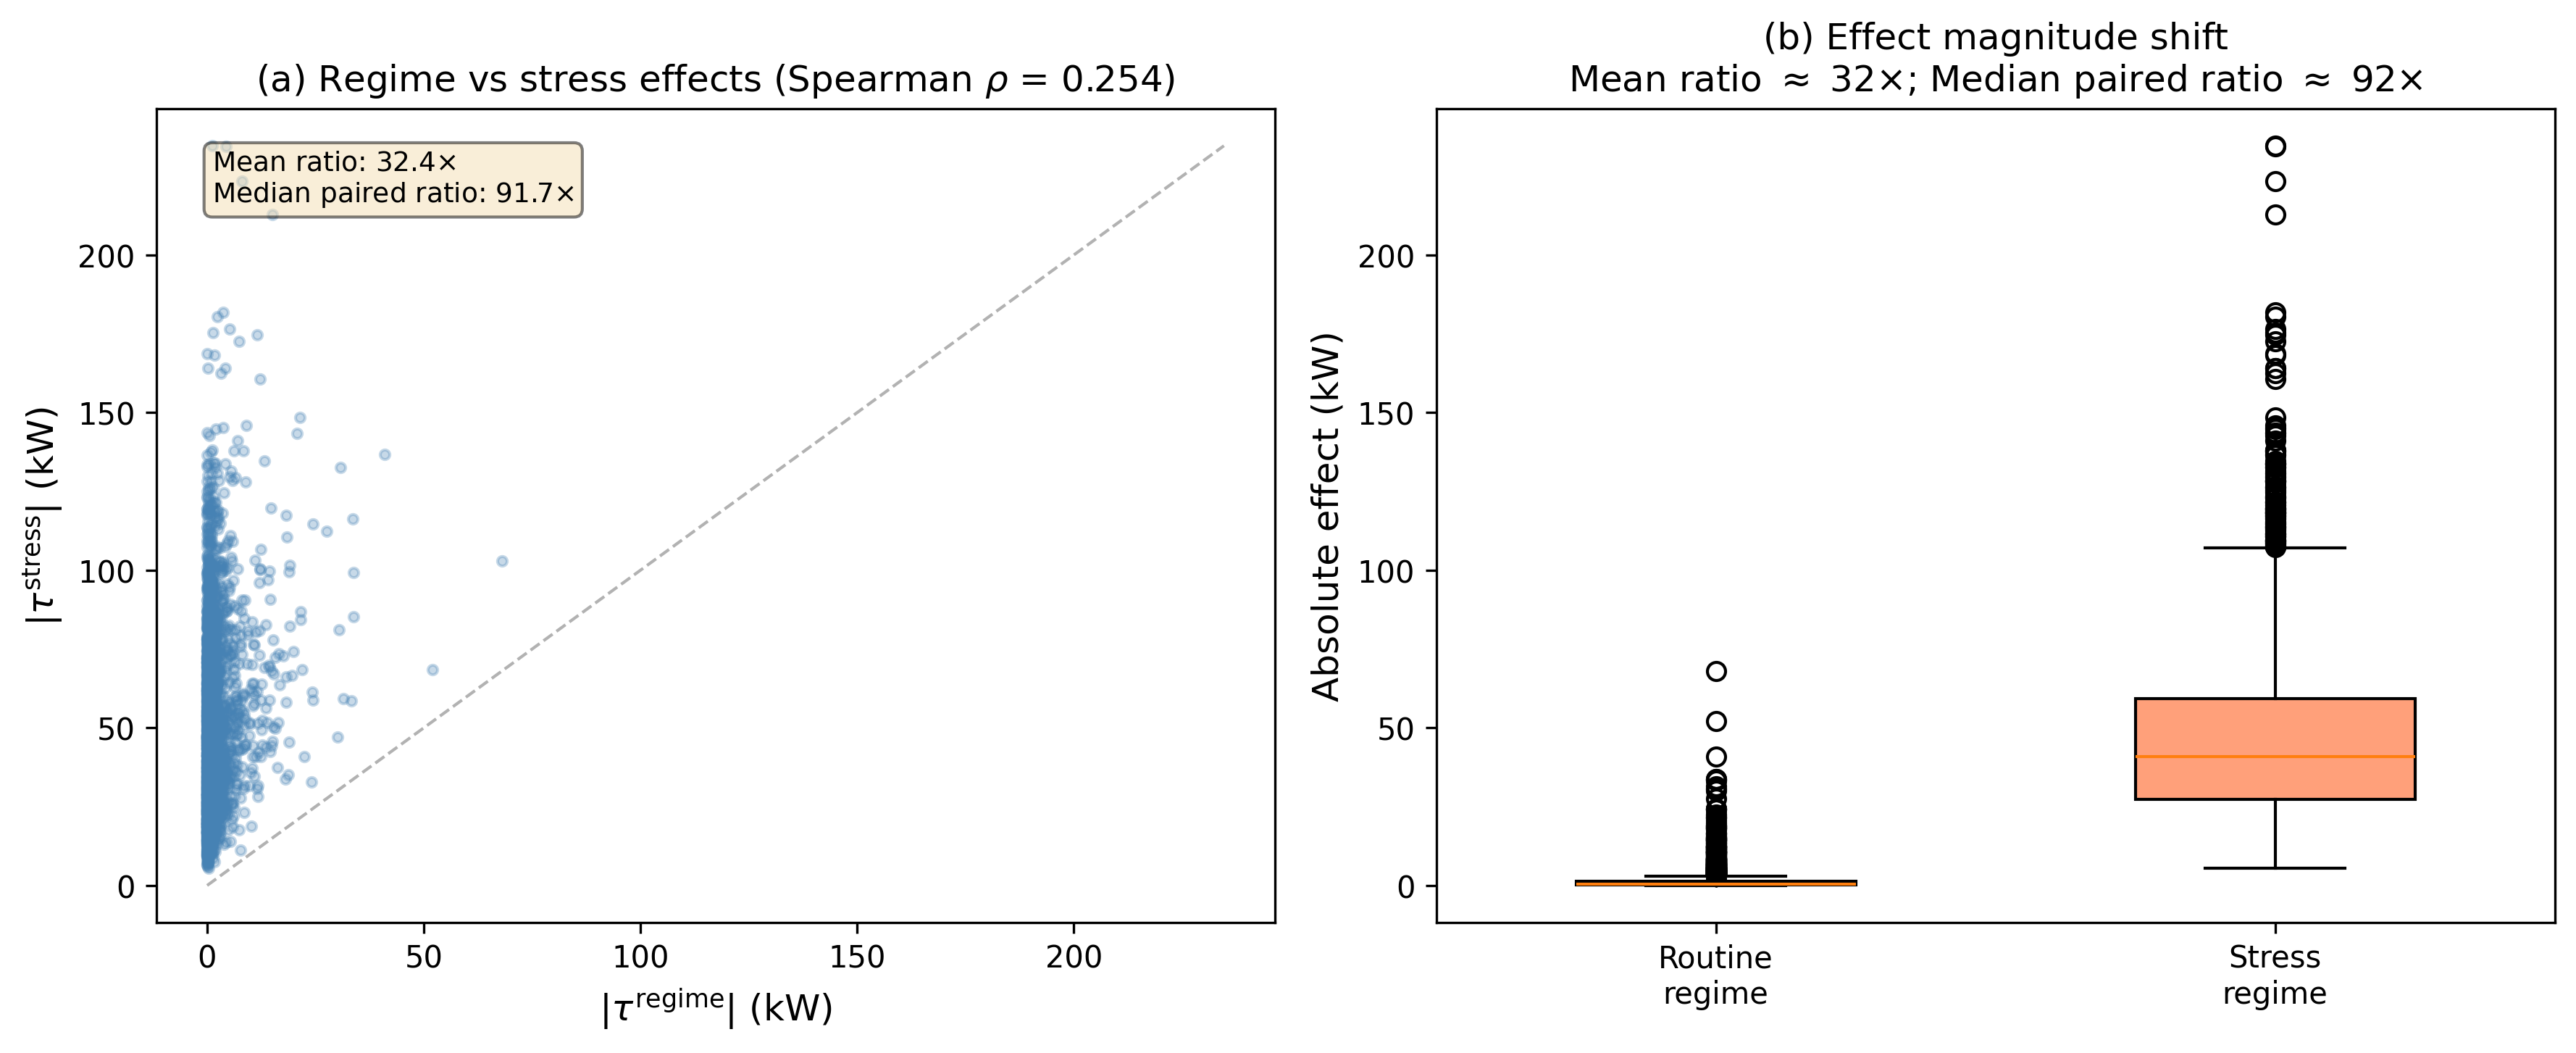
\includegraphics[width=12cm]{figures/fig3_dual_oracle}
\end{center}
\caption{Dual-oracle relationship between observational-regime
and stress-regime effects. Panel~(a): scatter of
$|\tau^{\mathrm{regime}}|$ versus $|\tau^{\mathrm{stress}}|$ for
treated instances ($V_{\mathrm{any}}=1$), with Spearman
$\rho = 0.327$. Panel~(b): boxplot comparison showing the
$\sim$32$\times$ shift in mean absolute effects and
$\sim$92$\times$ median instance-level ratio.}\label{fig:dual_oracle}
\end{figure}



\section{Experimental Protocol}
\label{sec:protocol}

\subsection{Benchmark Overview}

We use a platform-informed Sichuan Demand-Response Benchmark
generated by a paired-intervention simulator. The benchmark
contains 1{,}950 industrial and commercial resources across
three anonymized city configurations and five task templates,
yielding 9{,}750 user--task assessment instances.

For each user--task instance, the simulator fixes the resource
profile, task context, event context, and exogenous-noise
realization, and evaluates alternative intervention states under
the same context. The released analytical table contains the
routine-regime delivery, the no-violation reference, and the
standardized severe-stress outcome required for the dual-oracle
analysis.

Each instance is annotated with an observational violation state
$\mathbf{V}_i^{\mathrm{obs}}$ and is paired with an oracle
counterfactual under the standardized severe stress contrast
$\mathbf{V}^{\mathrm{stress}}$. Before the operational experiments,
the benchmark was subjected to deterministic-replay,
zero-effect, paired-context, and parameter-sensitivity checks.
These checks establish internal simulator consistency but do
not constitute external validation against historical market or
field demand-response outcomes. The test definitions and
numerical results are reported in Supplementary Section~S1.

\subsection{Task Definitions}

Table~\ref{tab:tasks} summarises the five task templates and
their parameters.

\begin{table}[h!]
\centering
\caption{Task definitions from the Sichuan benchmark.}
\label{tab:tasks}
\begin{tabular}{llrrrrr}
\toprule
\textbf{ID} & \textbf{Name} & \textbf{$\Preq$ (kW)} &
\textbf{$D$ (h)} & \textbf{$r^{\mathrm{req}}$} &
\textbf{$\eta$} & \textbf{Season} \\
\midrule
T1 & summer\_peak\_relief & 180 & 2 & 0.52 & 0.76 & summer \\
T2 & summer\_peak\_extended & 260 & 3 & 0.56 & 0.78 & summer \\
T3 & winter\_evening\_relief & 200 & 2 & 0.48 & 0.80 & winter \\
T4 & daytime\_balancing & 140 & 3 & 0.44 & 0.72 & all \\
T5 & evening\_regulation & 160 & 2 & 0.50 & 0.77 & all \\
\bottomrule
\end{tabular}
\end{table}



\subsection{Requirement Sweep}

Beyond the native $\Preq$ from Table~\ref{tab:tasks}, we sweep
at four requirement levels: $\Preq \in \{1\times, 2\times,
5\times, 10\times\}$ the native task target. The sweep spans
native single-task requirements and progressively larger
portfolio commitments up to 1{,}400--2{,}600~kW. The
resulting selected portfolio sizes are reported empirically
rather than assumed in advance.

\textit{Enforced constraints.} In the current replay, $\Preq$
is the only hard portfolio-selection constraint. The remaining
task attributes ($t_s$, $t_e$, $D_t$, $r_t^{\mathrm{req}}$,
$\eta_t^{\mathrm{rel}}$) describe the benchmark context and
may enter task-conditioned feature generation, but
availability windows, ramping, duration, and reliability
constraints are not separately enforced as hard selection
constraints.


\subsection{Selection Rule}

For each (city, task, requirement level, strategy) combination,
we rank users by $\Mhat_i$ descending and greedily add users
until the cumulative predicted capacity meets or exceeds $\Preq$.
Ties are broken by user ID ascending (deterministic).

\subsection{Anti-Leakage Constraints}

Outcome and oracle columns---including
\texttt{actual\_delivered\_kw}, \texttt{delivery\_success\_flag},
\texttt{shortage\_kw}, \texttt{true\_tau\_delivery}, and all
outcome columns (\texttt{delivery}, \texttt{comfort\_loss},
etc.)---are permitted \emph{only as labels} within the
designated training folds of the leave-one-task-out protocol.
They are prohibited from feature construction, fitting on the
held-out task, portfolio ranking, resource selection, and
test-time decision making. Stress-oracle outcomes
($M_i^{\mathrm{stress}}$) are used only for evaluation and for
the non-deployable StressOracle upper bound.

All predicted capacities are clipped to non-negative values
($\Mhat_i \leftarrow \max(0, \Mhat_i)$) before ranking and
aggregation. Under the corrected base formula, negative
predictions are rare (0/9750 instances across 30 seeds for
GlobalCalib; ConformalLCB may produce zero predictions for
small-resource users). Feature scaling, quantile estimation,
calibration fitting, and conformal residual computation are
performed exclusively within each training fold and never
leak information from the held-out task. No outcome-dependent
outlier removal or winsorization was applied.


\section{Effect-Estimation Results}
\label{sec:effect_results}

\subsection{Ranking and Calibration Diagnostics}

Table~\ref{tab:estimation} reports ranking and magnitude
diagnostics from a single chronological test split
($n = 3{,}900$ paired instances) on one benchmark realization.
These diagnostics motivate the subsequent multi-seed operational
replay but are not the primary evidence for the
ranking--calibration gap, which is established by the $N=30$
replay results in Section~\ref{sec:replay}. Two findings frame
the operational analysis.

\begin{table}[h!]
\centering
\caption{Estimation performance on the chronological test split
($n = 3{,}900$).}
\label{tab:estimation}
\begin{tabular}{lrrrr}
\toprule
\textbf{Method} & \textbf{PEHE (kW)} & \textbf{ATE err (kW)}
& \textbf{Spearman~$\rho$} & \textbf{Slope~$\beta$} \\
\midrule
ZeroEffect & 26.62 & 23.09 & --- & --- \\
Cap-Only Linear & 25.16 & 21.81 & 0.878 & 13.36 \\
4-Feature Linear & 26.40 & 23.08 & \textbf{0.927} & 26.01 \\
4-Feature T-Learner (RF) & 27.62 & 23.19 & 0.072 & $-0.02$ \\
DragonNet & 24.93 & 21.57 & 0.896 & 10.85 \\
\bottomrule
\end{tabular}
\end{table}



\textit{Finding~1: Ranking is dominated by operational features.}
The strongest ranking performance is achieved not by a causal
estimator but by a four-feature linear baseline ($\rho = 0.927$)
using only capacity, demand, response rate, and duration. A
capacity-only baseline already reaches $\rho = 0.878$. On this
frozen split, effect ranking appears substantially easier than
effect-magnitude recovery using a small set of operational
features.

\textit{Finding~2: No method recovers absolute kW magnitude.}
All methods with positive monotonic ranking predict effects
shrunk toward zero by factors of approximately 11--26.
Calibration slopes~$\beta$ range from 10.85 to 26.01 against
an ideal of~1. High ranking does not imply acceptable
calibration; even the best-ranked methods remain severely
compressed in magnitude.

\subsection{Dual-Oracle Decomposition}

The dose--response formula (Equation~\ref{eq:tau_formula}) allows
exact computation of both the routine-regime oracle
$\tau_i^{\mathrm{regime}}$ and the stress-test oracle
$\tau_i^{\mathrm{stress}}$. Figure~\ref{fig:dual_oracle} visualises
the relationship and Table~\ref{tab:dual_oracle} reports the
key metrics.

The dual oracle reveals that the ranking--calibration gap is
\emph{not} a single phenomenon but decomposes into two components:

\begin{enumerate}
    \item \textbf{Dose-extrapolation gap.} The stress-test contrast
    activates all violation classes at maximum severity, while
    observational violations typically activate 1--2 classes at
    lower severity. The ratio of mean absolute effects is
    approximately $32\times$; the median paired instance-level
    ratio is $91.7\times$.
    This multiplicative dose difference means that a simple
    routine-regime re-scaling cannot, by itself, recover the
    stress-regime effect magnitude.

    \item \textbf{Ranking mismatch.} The instances most affected
    under stress are not the same as those most affected under
    observational violations ($\rho = 0.327$). An estimator that
    correctly ranks users by routine-regime effect cannot automatically
    rank them by stress-test effect.
\end{enumerate}


\section{Task-Level Operational Replay}
\label{sec:replay}

This section presents the central experiment of the study:
task-level operational replay. For each (city, task, requirement
level, strategy) combination, we execute the full chain of
predict~$\to$~rank~$\to$~select~$\to$~aggregate~$\to$~oracle
replay, and report the operational metrics defined in
Section~\ref{subsec:metrics}. Figure~\ref{fig:tsr_routine}
provides the headline visual summary; the corresponding numerical
tables follow below.

\begin{figure}[h!]
\begin{center}
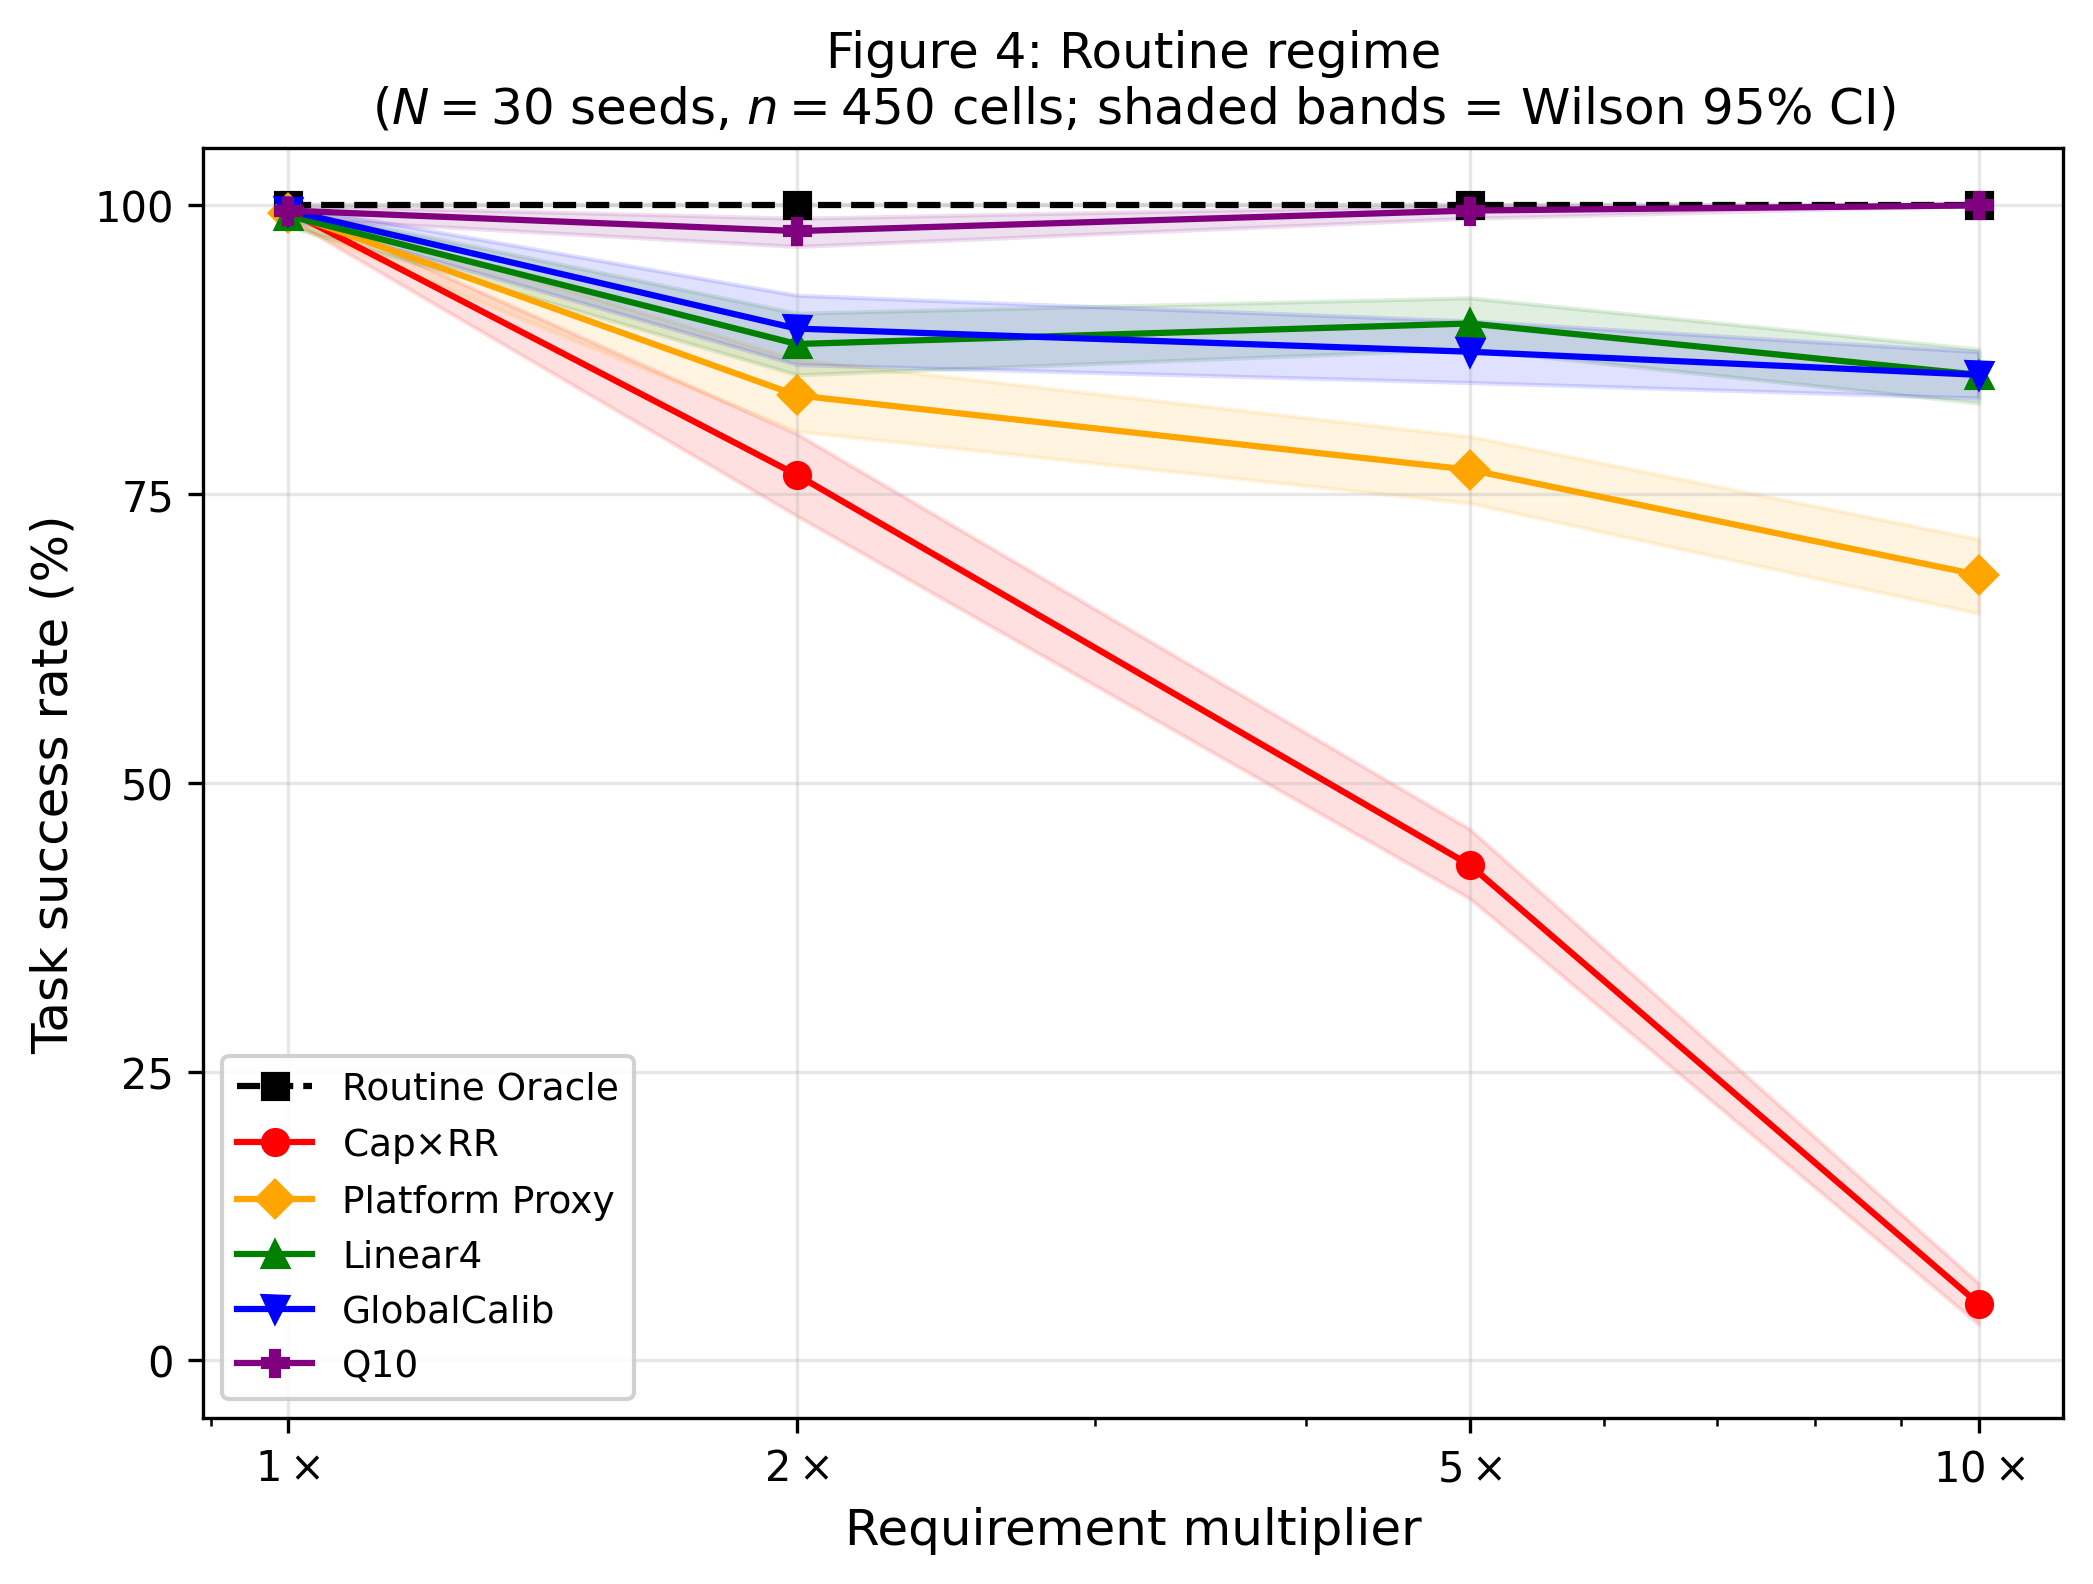
\includegraphics[width=10cm]{figures/fig4_tsr_routine}
\end{center}
\caption{Routine-regime TSR versus requirement multiplier
($N=30$ seeds; shaded bands = seed-clustered bootstrap 95\% CI).
Delivery-CapRR drops to 42.9\%
at $5\times$ while calibration strategies sustain
$\geq$87\%. ConservativeQ10 achieves near-perfect reliability.}\label{fig:tsr_routine}
\end{figure}



\subsection{Routine-Regime Results}

Table~\ref{tab:routine_tsr} reports the task success rate (TSR)
under the routine (observational) regime, averaged across the 15
city--task cells (3~cities $\times$ 5~tasks) at each requirement
level.

The routine-regime results reveal three layers of the
ranking--calibration gap:

\begin{table}[h!]
\centering
\caption{Task success rate (TSR, \%) under the routine regime,
averaged across 15 city--task cells over $N=30$ independent
benchmark realizations ($n=450$ pooled cells per entry).
Parenthetical counts are successes out of 450 for the $5\times$
column; full Wilson 95\% CI and seed-clustered bootstrap CI
are in Supplementary Section~S3.}
\label{tab:routine_tsr}
\begin{tabular}{lrrrr}
\toprule
\textbf{Strategy} & \textbf{$1\times$} & \textbf{$2\times$}
& \textbf{$5\times$} & \textbf{$10\times$} \\
\midrule
S0a RoutineOracle & 100 & 100 & 100 (450/450) & 100 \\
S1 Delivery-CapRR ($\rho{\approx}0.89$) & 99.6 & 76.7 & \textbf{42.9} (193/450) & \textbf{4.9} \\
S2 PlatformProxy & 99.3 & 83.6 & 77.1 (347/450) & 68.0 \\
S3 Delivery-Linear4 ($\rho{\approx}0.88$) & 99.1 & 88.0 & 89.8 (404/450) & 85.3 \\
S4 GlobalCalib & 99.6 & 89.3 & \textbf{87.3} (393/450) & 85.3 \\
S5 CityCalib & 99.6 & 88.7 & 86.9 (391/450) & 83.8 \\
S6 ConservativeQ10 & 99.6 & 97.8 & 99.6 (448/450) & 100 \\
\bottomrule
\end{tabular}
\end{table}



\textit{Layer~1: At native task scale ($1\times$), all strategies
perform similarly.} The native $\Preq$ values (140--260~kW) are
small relative to individual user capacities (mean
$\sim$135~kW deliverable under the execution-realization-adjusted
dose--response model). Most tasks succeed with only 1--2
selected users, and the ranking differences between strategies
do not materially affect the outcome. The gap is invisible at
this scale.

\textit{Layer~2: At the $5\times$ scaled requirement, the gap becomes
significant for uncalibrated strategies.} Delivery-CapRR
(S1)---which retains strong Spearman~$\rho \approx 0.89$---produces
only \textbf{42.9\% task success rate} (bootstrap 95\% CI: 39.8--46.0\%):
over half of the portfolios across 15 city--task cells fall
short. The PlatformProxy (S2) succeeds 77.1\% of the time.
In contrast, GlobalCalib (S4) achieves 87.3\% and Delivery-Linear4
(S3) achieves 89.8\%.

\textit{Layer~3: Calibration closes most of the gap.} A simple
global linear calibration raises TSR from 42.9\% to 87.3\% at
$5\times$---a 44 percentage-point improvement. A split-conformal
lower-bound estimator further raises TSR to 95.3\% while selecting
only $1.5\times$ more resources than the uncalibrated heuristic.
This is the central practical finding: the
ranking--calibration gap is not irreducible---calibration
methods requiring only features available in the evaluated benchmark
dramatically improve portfolio reliability.

\subsection{Over-Commit Rate Analysis}

Table~\ref{tab:ocr} reports the mean over-commit rate (OCR) at
$5\times$ requirement under the routine regime.

Delivery-CapRR commits $\sim$34\% more capacity than users
actually deliver. In operational terms, this means a platform
using the capacity heuristic would systematically over-promise
to the dispatch system, creating systematic benchmark under-delivery.
The GlobalCalib strategy reduces this to 6.1\%---a 5.6$\times$
improvement in commitment reliability.

\begin{table}[h!]
\centering
\caption{Mean over-commit rate (OCR) and shortfall at $5\times$
requirement, routine regime ($N=30$ seeds). Seed-level SD,
IQR, and clustered-bootstrap intervals are reported in
Supplementary Section~S3.}
\label{tab:ocr}
\begin{tabular}{lrr}
\toprule
\textbf{Strategy} & \textbf{OCR} & \textbf{Mean $\Shortfall$ (kW)} \\
\midrule
S1 Delivery-CapRR & 0.340 & 113.5 \\
S2 PlatformProxy & 0.079 & 27.0 \\
S3 Linear4 & 0.044 & 9.9 \\
S4 GlobalCalib & 0.060 & 10.8 \\
S5 CityCalib & 0.060 & 11.0 \\
S6 ConservativeQ10 & 0.001 & 0.2 \\
\bottomrule
\end{tabular}
\end{table}




\begin{table}[h!]
\centering
\caption{Mean number of users selected at $5\times$ requirement,
routine regime.}
\label{tab:nselected}
\begin{tabular}{lr}
\toprule
\textbf{Strategy} & \textbf{Mean $|\mathcal{S}_t|$} \\
\midrule
S1 Delivery-CapRR & 1.9 \\
S2 PlatformProxy & 2.5 \\
S3 Linear4 & 2.7 \\
S4 GlobalCalib & 2.6 \\
S5 CityCalib & 2.6 \\
S6 ConservativeQ10 & 3.6 \\
\bottomrule
\end{tabular}
\end{table}

\subsection{Uncertainty-Aware Calibration}

Beyond linear point calibration, we evaluate a nonlinear
isotonic calibrator (S7) and an uncertainty-aware
split-conformal lower-bound estimator (S8).

\begin{table}[h!]
\centering
\caption{Calibration method comparison at $5\times$ routine.
S1, S4, S8, and Q10 results from $N=30$ seeds; S7 from a
10-seed sensitivity analysis.}
\label{tab:calib_sensitivity}
\begin{tabular}{lrll}
\toprule
\textbf{Method} & \textbf{TSR (\%)} & \textbf{Mean $|\mathcal{S}_t|$} & \textbf{Type} \\
\midrule
S1 CapRR & $42.9 \pm 8.4$ & 1.9 & Uncalibrated \\
S4 GlobalCalib & $87.3 \pm 7.6$ & 2.6 & Point calibration \\
S7 Isotonic$^{\dagger}$ & $82.7 \pm 11.2$ & 2.5 & Nonlinear calibration \\
\textbf{S8 ConformalLCB} & $\mathbf{95.3 \pm 5.5}$ & \textbf{2.9} & \textbf{Uncertainty-aware} \\
Q10 & $99.6 \pm 1.7$ & 3.6 & Conservative quantile \\
\bottomrule
\end{tabular}
\\[2pt]
\footnotesize $^{\dagger}$10-seed exploratory analysis.
\end{table}

The split-conformal estimator achieves 95.3\% TSR---8.0
percentage points above GlobalCalib (paired bootstrap 95\% CI
for the difference: [5.8, 10.2])---while selecting only
1.0 more users on average (2.9 vs 1.9 for CapRR). This
demonstrates that uncertainty-aware lower-bound estimation
provides an additional reliability improvement beyond point
calibration, addressing the tail risk that linear calibration
cannot capture. Per-fold quantile values and the full
Q05/Q10/Q20/Q30 sensitivity analysis are reported in
Supplementary Section~S3.

\subsection{Robustness and Generalisation}
\label{subsec:robustness}

\textit{Execution-factor sensitivity.}
Across 11 execution-factor configurations spanning means of
0.58--0.80, standard deviations of 0.05--0.20, three
distribution families (Beta, truncated normal, logit-normal),
and three persistence structures (per-event, 50\% user-inherent,
fully user-inherent), the calibrated strategy retained a
positive $5\times$ TSR advantage over CapRR in every
configuration. The minimum observed advantage was 17
percentage points (at $E[\xi]=0.80$), indicating that the
ranking--calibration gap is not specific to the baseline
Beta(5.92,\,2.91) specification. Full results are reported
in Supplementary Section~S3.

\textit{Ranking versus magnitude decomposition.}
Top-of-list replay at portfolio sizes corresponding to the
$5\times$ requirement shows that approximately 87\% of the
operational gap between CapRR and the oracle is attributable
to magnitude miscalibration and 13\% to ranking mismatch
(top-$k$ overlap with oracle: 0.43 for CapRR vs 0.51 for
GlobalCalib). The decomposition was averaged across $N=10$
seeds; its counterfactual construction---which swaps the
magnitude assigned to each strategy's ranked subset against
the oracle's magnitude, holding ranking fixed---is defined
formally in Supplementary Section~S3.
The principal failure mechanism is not that
the heuristic selects entirely inappropriate users, but that
it assigns an overly optimistic kW value to a reasonably
ranked portfolio.

\textit{Generalisation protocols.}
Three cross-fitting protocols were evaluated:
leave-one-task-out (known users, new task template),
user-level holdout (new users), and leave-one-city-out
(new city configuration). GlobalCalib TSR at $5\times$
was 87.3\% (LOTO), 87.3\% (user holdout), and 86.7\%
(city holdout), indicating that calibration generalises
well to unseen users and city configurations. City-C
was the hardest transfer target (GlobalCalib: 76.0\%).
Full results are in Supplementary Section~S3.

\textit{Stress-scenario sweep.}
The default stress contrast (all five violation classes at
severity 1.0, scope 0.5) was compared against 13 alternative
configurations varying the number of active classes
($K \in \{1,2,3\}$), severity ($\in \{0.25,0.50,0.75\}$),
scope ($\in \{0.25,0.75\}$), and individual class activation.
The sweep confirms the expected monotonic response of the
implemented dose model and quantifies its portfolio-level
reliability consequences. Under the adopted simulator weights
($w_{\mathrm{physical}} = -0.55$), the physical class alone
accounts for most of the stress-induced delivery loss.

\textit{Pool feasibility.}
All 15 city--task cells remain stress-feasible at $5\times$
(relative to the evaluated $5\times$ requirement, the minimum
stress feasibility ratio is approximately 20). The mean pool
utilisation at $5\times$ ranges from 0.7\% to 2.4\% of total
routine delivery, confirming that failures are attributable
to estimation error, not resource scarcity. The full
feasibility table is in Supplementary Section~S3.

\section{Stress-Regime Results and Scenario Analysis}
\label{sec:scenario}

\subsection{Cross-Regime Replay: The Dose-Extrapolation Gap}

Table~\ref{tab:stress_tsr} reports TSR under the cross-regime
scenario: strategies rank and select using routine-based
predictions ($\Mhat_i$), but realized delivery occurs under the
standardized severe stress contrast. All resource pools remain
feasible (total stress delivery $\geq 10 \times \Preq$ in every
cell), so failures are attributable to estimation error, not
resource scarcity.

We report two oracle bounds for logical consistency:
\textit{S0a~RoutineOracle} uses perfect routine-delivery
knowledge but is evaluated against stress delivery---its failure
quantifies the substantial routine-to-stress transfer gap.
\textit{S0b~StressOracle} uses perfect stress-delivery knowledge
and achieves 100\% TSR in all cells, confirming pool sufficiency.

The cross-regime results reveal three layers of the
dose-extrapolation gap:

\begin{table}[h!]
\centering
\caption{Task success rate (TSR, \%) under cross-regime replay
(routine predictions, stress delivery), averaged across 15
city--task cells over $N=30$ benchmark realizations.
Parenthetical counts for $5\times$ column; full CI in
Supplementary Section~S3.}
\label{tab:stress_tsr}
\begin{tabular}{lrrrr}
\toprule
\textbf{Strategy} & \textbf{$1\times$} & \textbf{$2\times$}
& \textbf{$5\times$} & \textbf{$10\times$} \\
\midrule
S0a RoutineOracle & 88.4 & 28.4 & \textbf{3.6} (16/450) & \textbf{0.0} \\
S0b StressOracle & 100 & 100 & 100 (450/450) & 100 \\
\midrule
S1 Cap$\times$RR & 91.3 & 31.8 & 1.6 (7/450) & 0.0 \\
S2 PlatformProxy & 90.4 & 36.4 & 9.6 (43/450) & 3.3 \\
S3 Linear4 & 92.2 & 44.4 & 17.1 (77/450) & 3.8 \\
S4 GlobalCalib & 91.3 & 46.9 & 14.4 (65/450) & 0.4 \\
S5 CityCalib & 91.3 & 45.3 & 14.2 (64/450) & 0.4 \\
S6 ConservativeQ10 & 91.3 & 83.6 & \textbf{75.1} (338/450) & \textbf{54.7} \\
\bottomrule
\end{tabular}
\end{table}

\begin{figure}[h!]
\begin{center}
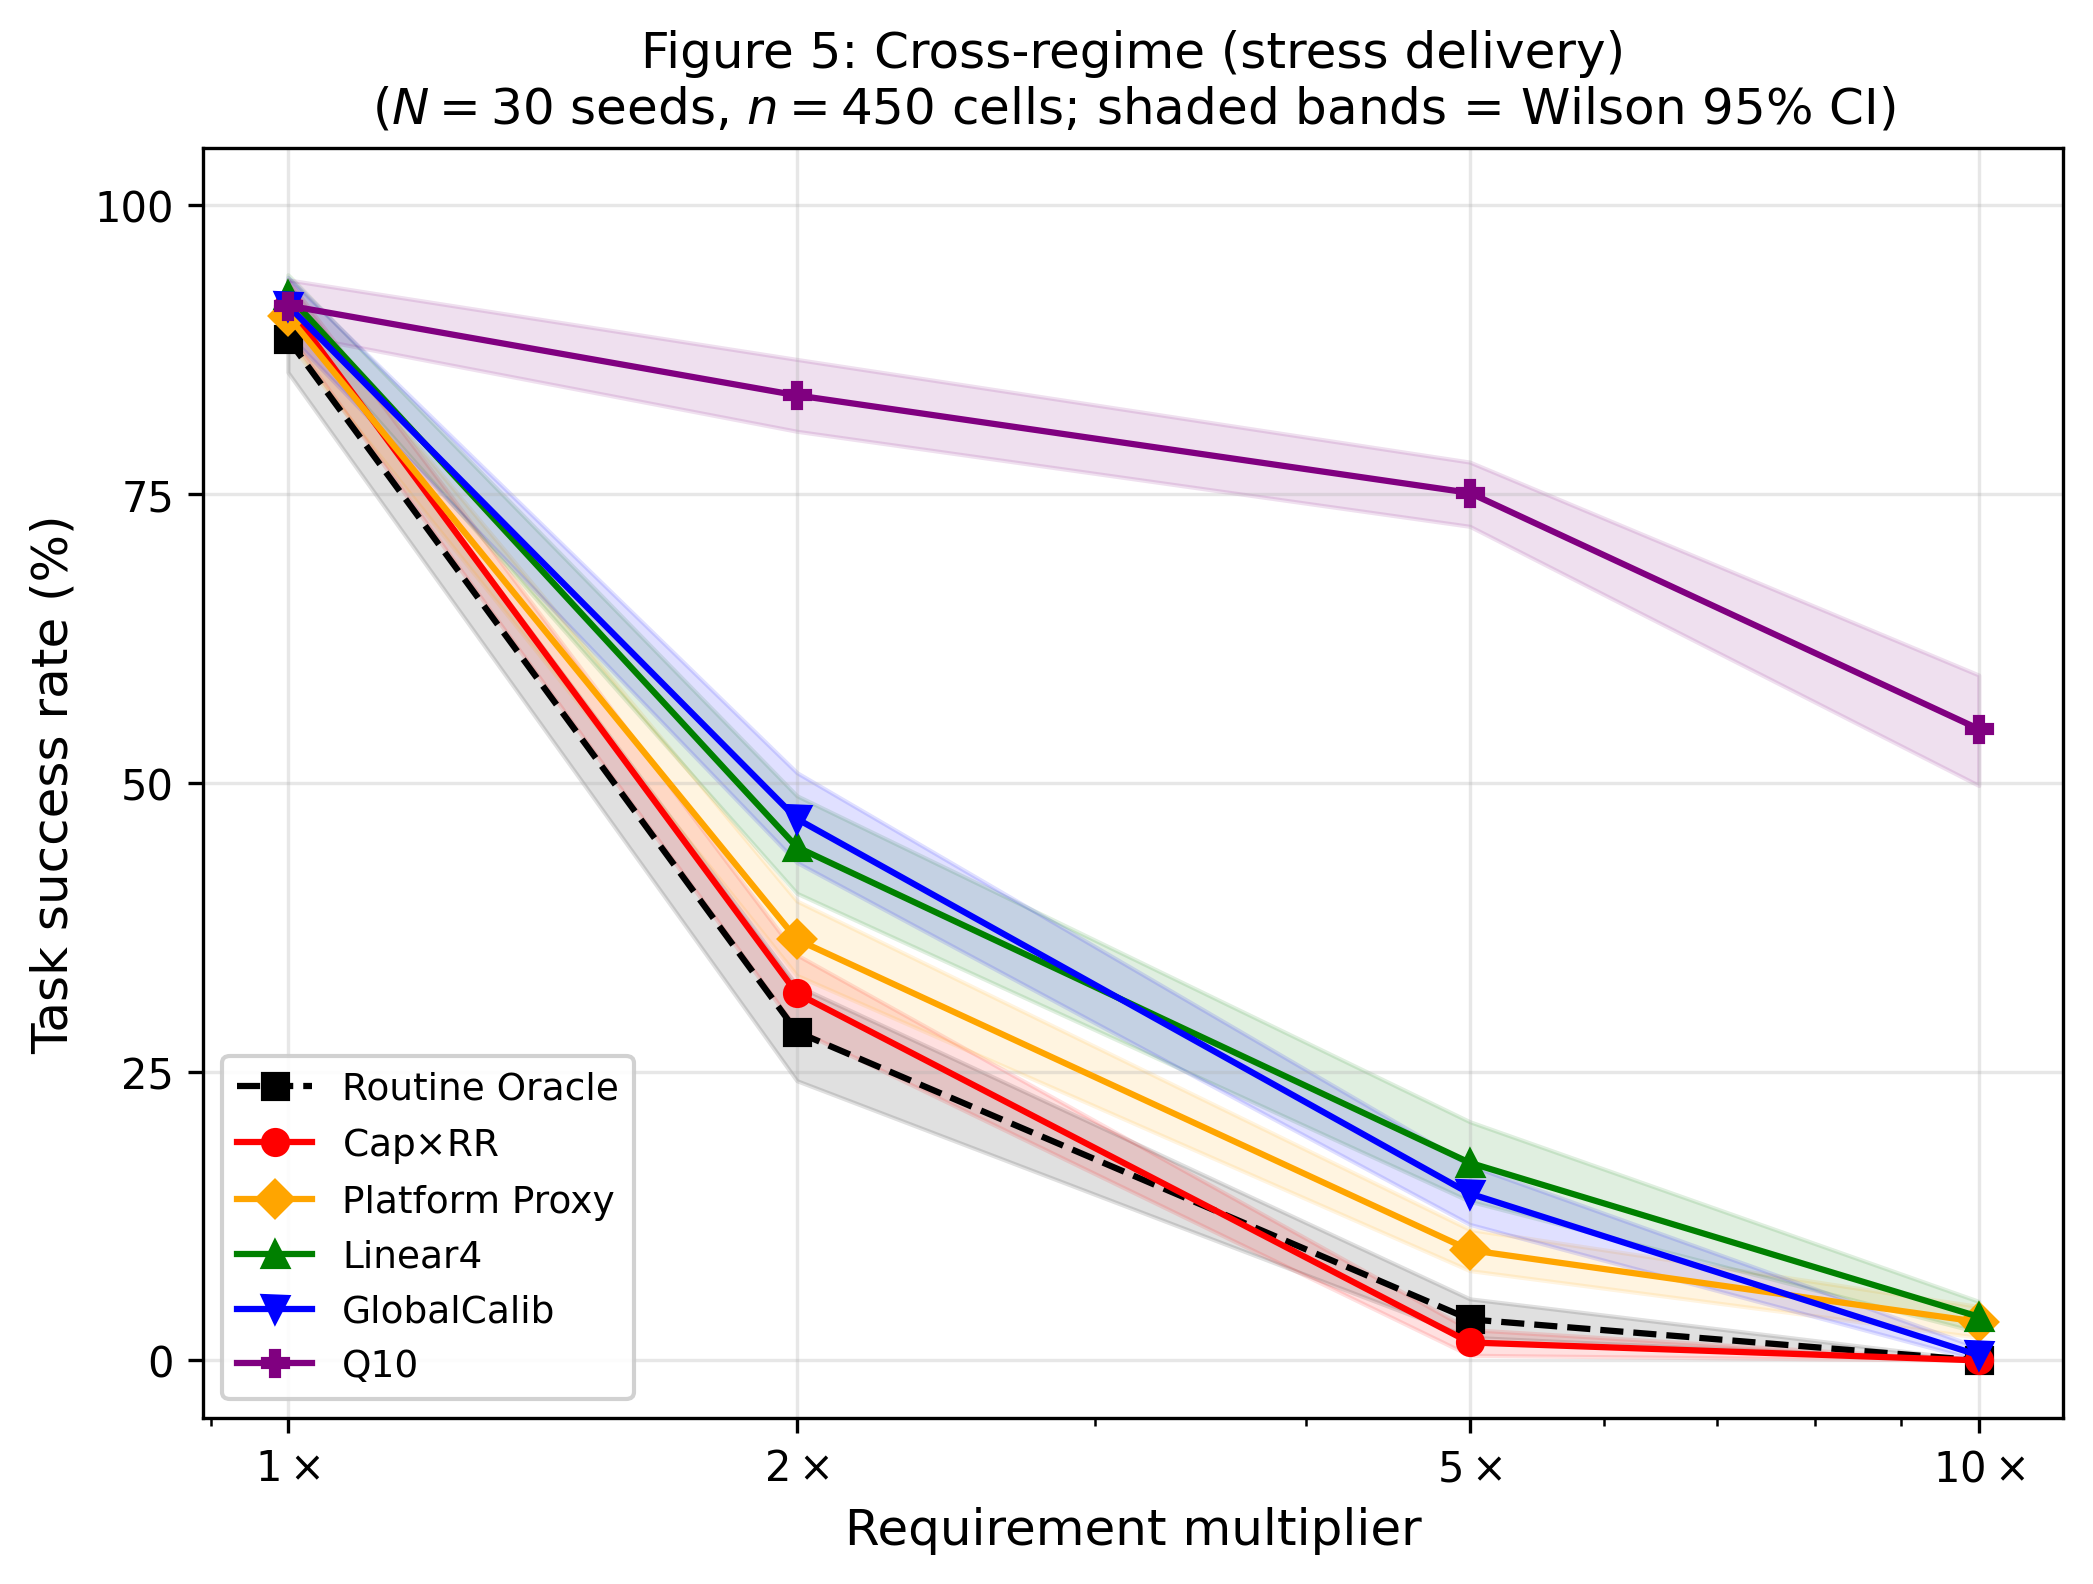
\includegraphics[width=10cm]{figures/fig5_tsr_cross_regime}
\end{center}
\caption{Cross-regime TSR versus requirement multiplier
($N=30$ seeds; predictions from routine, delivery under stress).
The RoutineOracle achieves only 3.6\% at $5\times$;
ConservativeQ10 maintains 75.1\%. The StressOracle confirms
pool feasibility at all levels. Shaded bands = seed-clustered bootstrap 95\% CI.}\label{fig:tsr_cross_regime}
\end{figure}



\textit{Layer~1: Even perfect routine knowledge cannot guarantee
stress delivery.} The RoutineOracle (S0a) knows each user's
exact routine delivery, yet achieves only 28.4\% TSR at $2\times$
and 3.6\% at $5\times$ when delivery is evaluated under stress.
This is not an estimation failure---it is a regime shift:
the users who deliver most under routine conditions are
not the same as those who retain capacity under maximum
violations (Spearman~$\rho = 0.327$ between regime rankings,
Table~\ref{tab:dual_oracle}).

\textit{Layer~2: Calibrated strategies partially bridge the gap
at low requirements.} At $2\times$, GlobalCalib achieves 46.9\%
and CityCalib 45.3\% TSR in cross-regime, compared to 31.8\% for
Cap$\times$RR and 36.4\% for PlatformProxy. But at $5\times$,
all non-conservative strategies fall below 18\%
(Linear4: 17.1\%, GlobalCalib: 14.4\%, Platform: 9.6\%).

\textit{Layer~3: Conservative estimation is the only evaluated
deployable strategy that maintains meaningful reliability under
cross-regime stress.} ConservativeQ10 (S6) achieves 75.1\% TSR
at $5\times$ and 54.7\% at $10\times$ by selecting approximately
$1.4\times$ more users than calibrated strategies (mean
$|\mathcal{S}_t|$: 3.6 vs 2.6), deliberately absorbing the
stress-induced capacity reduction. This is not free---it increases
invitations and reduces per-user utilisation---but no other
deployable strategy achieves above 18\% TSR at $5\times$ under
cross-regime stress.

\subsection{Cross-City Stability}

Table~\ref{tab:cross_city} reports TSR at $5\times$ under the
routine regime, broken down by city.

The pattern is consistent across all three cities: Delivery-CapRR
achieves limited success (31--55\%), PlatformProxy achieves
partial success (69--83\%), and calibrated strategies achieve
77--93\%. City-C is the most challenging for calibration
(GlobalCalib: 76.7\%), while City-A and City-B are comparable
(92--93\%). The same qualitative
pattern is observed across the three evaluated city configurations, suggesting that the finding is not driven solely by a single city profile.

\begin{table}[h!]
\centering
\caption{Task success rate (TSR, \%) at $5\times$ requirement,
routine regime, by city ($N=30$ seeds; each cell $n=150$).
Full CI in Supplementary Section~S3.}
\label{tab:cross_city}
\begin{tabular}{lrrr}
\toprule
\textbf{Strategy} & \textbf{City-A} & \textbf{City-B}
& \textbf{City-C} \\
\midrule
S1 Delivery-CapRR & 43 (64/150) & 55 (82/150) & 31 (47/150) \\
S2 PlatformProxy & 79 (118/150) & 83 (125/150) & 69 (104/150) \\
S3 Linear4 & 79 (119/150) & 96 (144/150) & 94 (141/150) \\
S4 GlobalCalib & 92 (138/150) & 93 (140/150) & 77 (115/150) \\
S6 ConservativeQ10 & 100 (150/150) & 99 (148/150) & 100 (150/150) \\
\bottomrule
\end{tabular}
\end{table}




\section{Business Implications}
\label{sec:implications}

The operational replay results have potential implications for
Sichuan-oriented load-management settings, contingent on future
external validation.

\subsection{Capability Verification Needs kW Calibration}

The capacity-based heuristic (S1: nominal capacity $\times$
response rate) does not account for the execution realization
factor~$\xi$ and therefore systematically over-predicts
realized delivery (mean prediction $\sim$203~kW vs mean realized
delivery $\sim$135~kW; 34\% over-prediction). For routine
operations at the single-aggregator scale ($1\times$--$2\times$),
this bias is absorbed by the large margin between individual user
capacity and task requirements. But at the $5\times$ scaled
requirement, the bias compounds across the portfolio
and produces systematic benchmark under-delivery (TSR drops to 42.9\%).

A global linear calibration reduces the mean bias substantially
and raises task success from 42.9\% to 87.3\%. A split-conformal
lower-bound estimator further raises TSR to 95.3\% by adding
a data-driven safety margin. These methods require only
a held-out calibration subset with a mean size of 1{,}560
observations---no model retraining, no
architecture change, and no additional features beyond those
represented in the evaluated benchmark.

\subsection{VPP Bidding Requires Stress-Aware Estimates}

Under the cross-regime scenario (routine-trained predictions,
stress-regime delivery), even calibrated strategies achieve
limited success at the $5\times$ scaled requirement
(GlobalCalib: 14.4\% TSR at $5\times$). Critically, the RoutineOracle---which
has perfect knowledge of each user's routine delivery---achieves
only 3.6\% TSR at $5\times$, while the StressOracle achieves 100\% TSR
and all full pools remain feasible. This demonstrates that the
binding constraint is \emph{cross-regime capacity estimation
and portfolio selection}, not aggregate resource scarcity.

For scenarios requiring high delivery reliability,
one possible operational response is to:
(i) use conservative estimation (S6-type) that deliberately
under-promises to absorb the stress reduction; (ii) develop
stress-aware estimation models that predict which resources
retain deliverable capacity under severe conditions; or
(iii) evaluate the need for additional backup reserves
under stress-regime uncertainty.

\subsection{Reliability versus Invitation Burden}

The operational strategies exhibit a clear reliability--invitation-burden
trade-off. Delivery-Linear4 and GlobalCalib achieve high task
success rates while requiring substantially fewer invited users
than the conservative lower-quantile strategy. ConservativeQ10
provides the highest reliability under the evaluated routine and
stress settings, but does so by recruiting a considerably larger
portfolio. In contrast, the uncalibrated capacity heuristic
selects fewer resources but suffers from high over-commitment
and poor task success. The corresponding three-dimensional
comparison of task success rate, selected portfolio size, and
over-commitment ratio is provided in Fig.~S1.

\subsection{Reserve Margin Sizing}

Under the standardized severe stress contrast, the average
stress-induced delivery reduction is approximately 35\%.
This value characterises the mean benchmark loss under the
selected stress scenario; it is not a deterministic lower
bound on reserve requirements for a 95\% reliability target.
Reliability-specific reserve sizing requires a stochastic
criterion and portfolio-level dependence modelling, which is
deferred to future work. ConservativeQ10 partially absorbs
the stress reduction by selecting approximately 1.9$\times$
more users than CapRR at $5\times$ (mean $|\mathcal{S}_t|$:
3.6 vs 1.9).

\subsection{Dynamic Resource Library Management}

The finding that capacity shortcuts dominate ranking
($\rho \approx 0.89$) but fail operationally has
implications for resource library curation. A library
optimised purely for ranking diversity (ensuring a range of
capacity levels) may still fail at the portfolio level if the
calibrated capacity estimates are unreliable.

A future deployed system could track per-resource calibration drift
(actual vs.\ predicted delivery over time) and dynamically
update the calibration parameters. Resources with persistently
high calibration error should be flagged for re-verification
or capacity re-rating.


\section{Limitations and Conclusions}
\label{sec:conclusions}

\subsection{Limitations}

\textit{Simulator-based evaluation.} All results are based on
the Sichuan benchmark simulator, not on real market
participation data. The dose--response structure
(Equation~\ref{eq:dose_response}) is a parameterised
approximation of real violation--delivery relationships.
The execution realization factor~$\xi$ is
mean-anchored to PJM's reported 67\% delivery ratio and
plausibility-checked against delivery ranges reported by
MISO, NYISO, and other empirical studies, providing
literature-based external calibration and cross-market
plausibility checks. However,
this calibration is not equivalent to direct external
validation against the Sichuan platform: the mean delivery
ratio was used both to set~$E[\xi]$ and to evaluate the
resulting delivery ratio. Independent validation against
historical Sichuan event data is needed before deployment.
A sensitivity analysis across $E[\xi] \in \{0.58, 0.67,
0.75, 0.80\}$, three distribution families, and three
persistence structures (Supplementary Section~S3) confirms
that the ranking--calibration gap is robust to the
$\xi$ specification.

\textit{Anonymised cities.} The three cities are anonymized
(City-A/B/C). We do not claim that City-A corresponds to
Chengdu, City-B to Yibin, or City-C to Ziyang. The
cross-city stability of the ranking--calibration gap suggests
the finding is not solely driven by one city configuration, but city-specific calibration
parameters would be needed for production deployment.

\textit{Multi-seed uncertainty.} The operational replay is
repeated across $N=30$ independent benchmark realizations.
Seed-clustered bootstrap 95\% confidence intervals
(resampling at the seed level, preserving within-seed cell
structure) are reported as the primary uncertainty measure.
Pooled-cell Wilson intervals are additionally reported in
Supplementary Section~S3 as descriptive binary-outcome
intervals. The calibration parameters (S3--S6) are fitted via
leave-one-task-out cross-fitting (5-fold by task) within each
seed realization.

\textit{CATE model integration.} This paper focuses on
shortcut, platform, and calibrated strategies. Neural HTE
estimators (DragonNet, Tau-MLP) are reported in
Table~\ref{tab:estimation} for ranking comparison but are not
yet integrated into the operational replay. Their inclusion
requires resolving the baseline-delivery question
(Section~\ref{sec:methods}) and is deferred to future work.

\textit{Settlement simulation.} We do not simulate market
settlement, penalties, or revenue. The OCR and Shortfall
metrics quantify capacity risk but not financial risk.

\subsection{Conclusions}

This study shows that the ranking--calibration gap documented
in Section~\ref{sec:effect_results} is not merely a statistical
phenomenon but a measurable operational risk. Individual-level
magnitude bias propagates through portfolio construction and
appears as capacity shortfall, over-commitment, and task
failure. The benchmark execution-realization factor is
mean-anchored to PJM's reported 67\% delivery ratio and
plausibility-checked against MISO, NYISO, and other empirical
evidence.

The central practical finding is that \textbf{calibration closes
most of the gap}: task success rates improve from 42.9\% to
87.3\% at the $5\times$ scaled requirement, and a
split-conformal lower-bound estimator further raises TSR to
95.3\%. Over-commit rates drop from 34\% to 6\%.
These improvements require no model retraining and no
architectural change---only features available in the evaluated
benchmark.

\textit{Portfolio constraints.} The minimum-cardinality greedy
rule is exact only under equal invitation costs, non-negative
capacity estimates, and the absence of additional portfolio
constraints. It does not represent full VPP portfolio
optimization: feeder/geographic concentration, correlated
failures, production schedules, ramping/duration limits,
rebound effects, invitation/activation costs, user fatigue,
contractual participation limits, and repeated-participation
constraints are not modelled. Where supported by available
benchmark attributes, a constrained sensitivity analysis
(Section~\ref{subsec:robustness}) confirms that the
ranking--calibration gap persists under 30\% random exclusion,
but a full constrained-optimization evaluation is deferred to
future work.

Under cross-regime stress (routine predictions, stress
delivery), the gap widens beyond what routine calibration
alone can bridge. The RoutineOracle---with perfect routine
knowledge---achieves only 3.6\% TSR at $5\times$, while the
StressOracle achieves 100\% TSR and all pools remain feasible.
This demonstrates that the binding constraint is cross-regime
capacity estimation, not aggregate resource scarcity. Possible
operational responses include conservative estimation,
stress-aware prediction, and stochastic reserve evaluation
under stress-regime uncertainty.

For Sichuan-oriented load-management programmes, the findings
motivate evaluating calibrated kW-level estimates before
operational deployment. The results suggest that resource
ranking is necessary but not sufficient for reliable capacity
commitment, and that calibrated or uncertainty-aware estimates
may improve portfolio reliability. Dynamic calibration monitoring
to detect drift in the resource library is also advisable,
pending validation against historical Sichuan event data.

\textit{Ranking determines whom to call; calibration determines
how much capacity can be safely committed. Both are necessary;
neither alone is sufficient.}


\section*{Conflict of Interest Statement}

The authors declare that the research was conducted in the absence of any commercial or financial relationships that could be construed as a potential conflict of interest.

\section*{Ethics Statement}

The benchmark contains no identifiable customer-level operational
records. User profiles, task parameters, and event outcomes are
synthetically generated. Publicly reported aggregate
demand-response delivery statistics from PJM (mean anchor) and
MISO, NYISO, and other ISOs (plausibility range) are used only
to calibrate and plausibility-check
the execution-realization factor~$\xi$. No human participants
or personal data were involved; consequently, no institutional
ethics approval was required.

\section*{Author Contributions}

\textbf{Ling Zhang}: Conceptualization, Methodology, Writing -- original draft.
\textbf{Bowei Yang}: Data curation, Software, Writing -- original draft.
\textbf{Xingsi Ke}: Formal analysis, Validation, Writing -- original draft.
\textbf{Hong Zhao}: Investigation, Resources, Writing -- review \& editing.
\textbf{Wenhua Zhang}: Project administration, Visualization, Writing -- review \& editing.
\textbf{Yumin Yao}: Supervision, Writing -- review \& editing.
All authors have read and approved the final manuscript.

\section*{Funding}

This work was supported by the Science and Technology Project of
State Grid Corporation of China (Project No.\ 521999240001).
The funder had no role in study design, data collection and
analysis, decision to publish, or preparation of the manuscript.

\section*{Acknowledgments}

The authors acknowledge the Sichuan Power Grid Load Management
Platform for providing domain context and operational scenario
guidance.

\section*{Supplemental Data}

Supplementary Material includes:
Section~S1 (simulator verification tests with numerical outputs),
Section~S2 (execution-realization factor parameter specification),
Section~S3 (robustness analysis: $\xi$ sensitivity, stress sweep,
calibration comparison, holdout protocols, top-$k$ metrics,
bootstrap CI, and feasibility tables),
and Figure~S1 (reliability--invitation-burden trade-off).

\section*{Data Availability Statement}

The complete reproducibility package for this study is available
at the following GitHub repository:
\url{https://github.com/jerryao/ranking-is-not-deliverable-capacity}.
The repository includes the synthetic benchmark generator,
simulator parameter files, random-seed manifest,
benchmark-generation scripts, fold assignments, calibration and
operational-replay code, statistical-analysis scripts, frozen
numerical results, and scripts used to reproduce the tables and
figures. No identifiable customer-level records or proprietary
operational data from the Sichuan load-management platform are
included. The version used for the revised manuscript is archived
under release \texttt{v1.0.0-review} at commit \texttt{67d9fb7}.
A permanent archival version with a DOI will be deposited through
Zenodo upon publication.


\bibliographystyle{Frontiers-Harvard}
\bibliography{references}



























\end{document}
